 \input{../Plantillas-Fomato/Tareas/tarea.tex}
\tcabe{Introducción a las Probabilidades}{Jhonny Lanzuisi, 1510759}
\cabe{Introducción a las Probabilidades: Tarea I}

\begin{document}
	\thispagestyle{plain}
\chapter*{Distribuciones Discretas}
	{\noindent En todos los ejercicios de esta tarea aparecerá primero la probabilidad calculada usando \texttt{Geogebra 6.0.535.0} ---con su respectiva gráfica--- y después la misma probabilidad calculada usando \texttt{R} (\texttt{r-base 3.5.2-1} en \texttt{Debian GNU/Linux})}. 
	\vspace{.5em}
	\subsection{Distribución de bernoulli}
	\begin{ejer}[0,5]
		Para la distribución Bernoulli, que es lo mismo que Binomial $(1, \theta)$, $P(X \leq 0)$ cuando $\theta = 0.83$.
	\end{ejer}
	\begin{sol}
		Por un lado, con los parámetros $n=1$ y $p=0.83$, \texttt{Geogebra} da una $P(X\leq 0) = 0.17$ con el siguiente gráfico:
		\begin{figure}[H]
			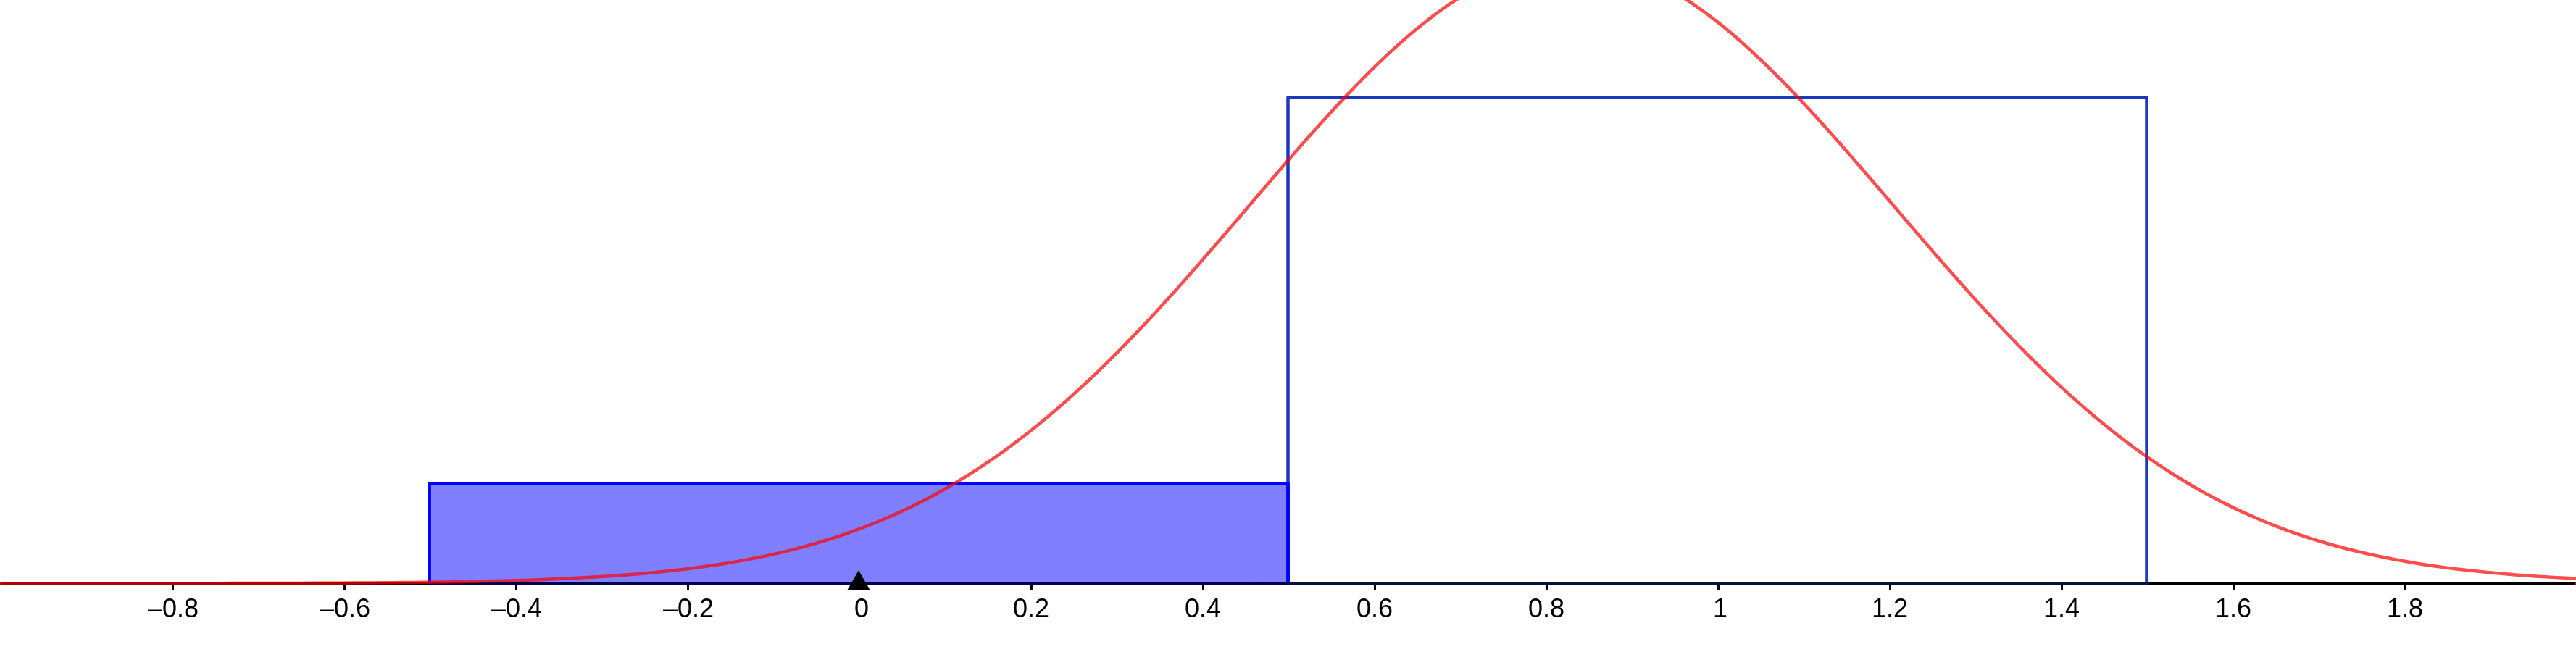
\includegraphics[width=0.5\linewidth]{pics/g1}
			\centering
		\end{figure}
		\noindent Por otro lado, en \texttt{R}, $P(X\leq 0)$ es:
		\begin{lstlisting}[language=R]
> pbinom(0, 1, 0.83, lower.tail = TRUE)
[1] 0.17
		\end{lstlisting}
	\end{sol}
\subsection{Distribución binomial}
\begin{ejer}[1]
	Para la distribución Binomial $(20, \theta = 0.7)$, $P(X \leq 10)$ y $P(14 \leq X \leq 18)$.
\end{ejer}
\begin{sol}
	Por un lado, con los parámetros $n=20$ y $p=0.7$, \texttt{Geogebra} da una $P(X\leq 10) = 0.048$ con el gráfico
	\begin{figure}[H]
		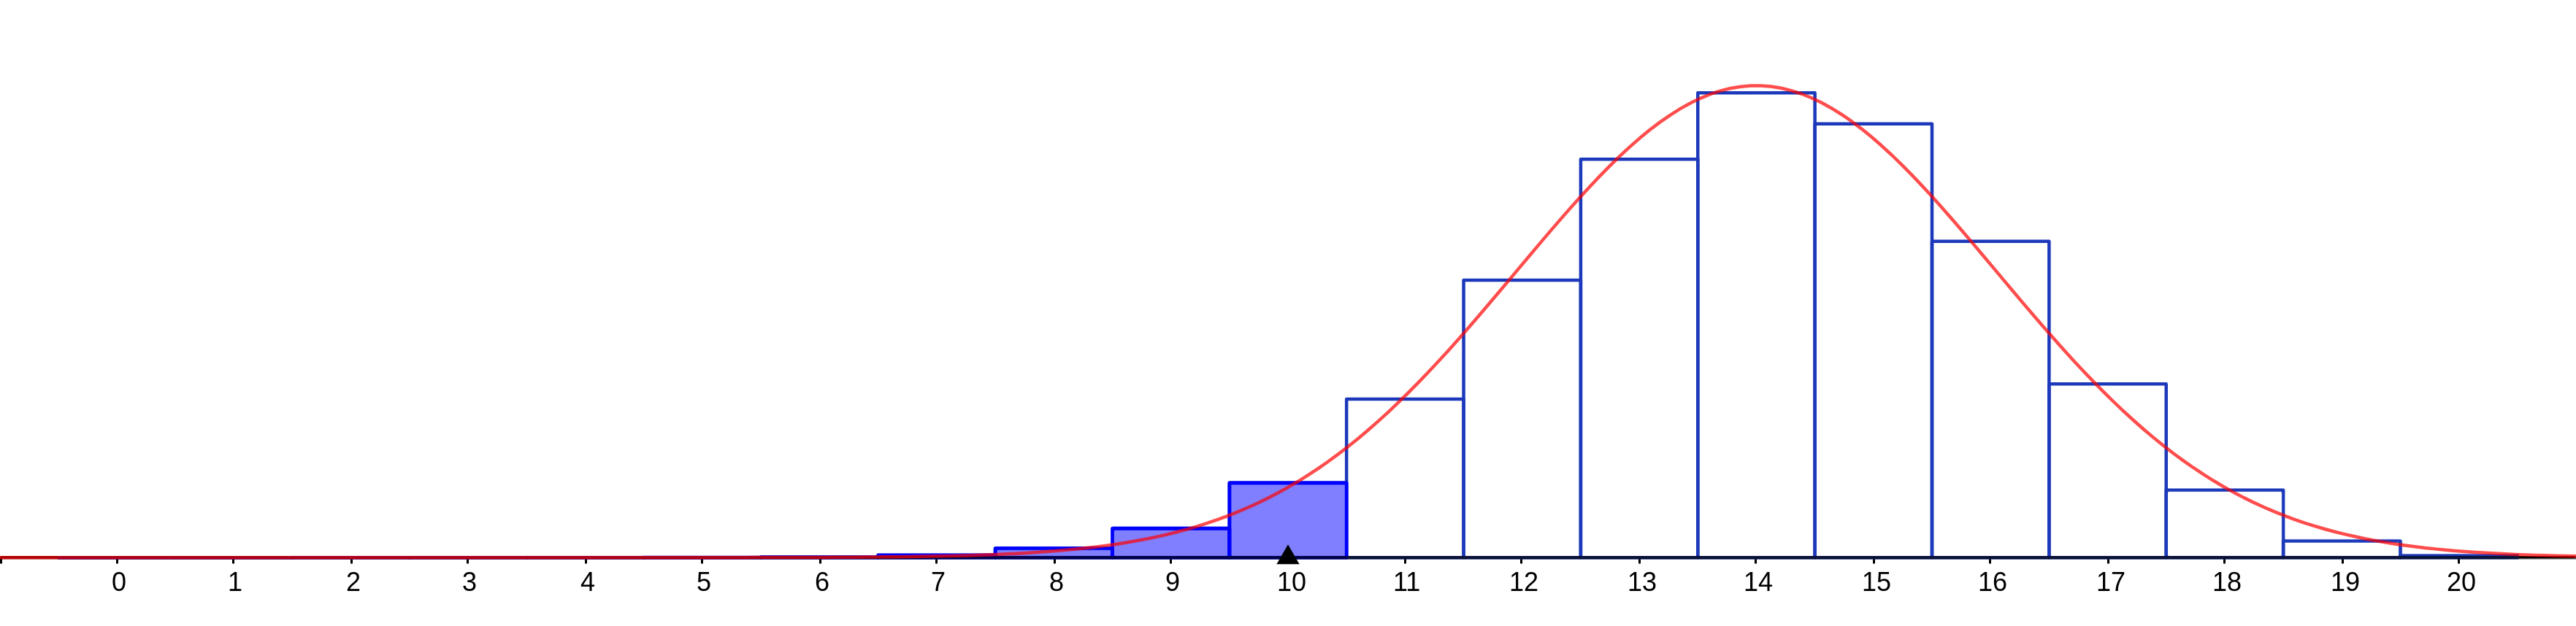
\includegraphics[width=0.5\linewidth]{pics/g2-1}
		\centering
	\end{figure}\noindent
%
	y $P(14 \leq X \leq 18) = 0.6004$ con el gráfico 
	\begin{figure}[H]
		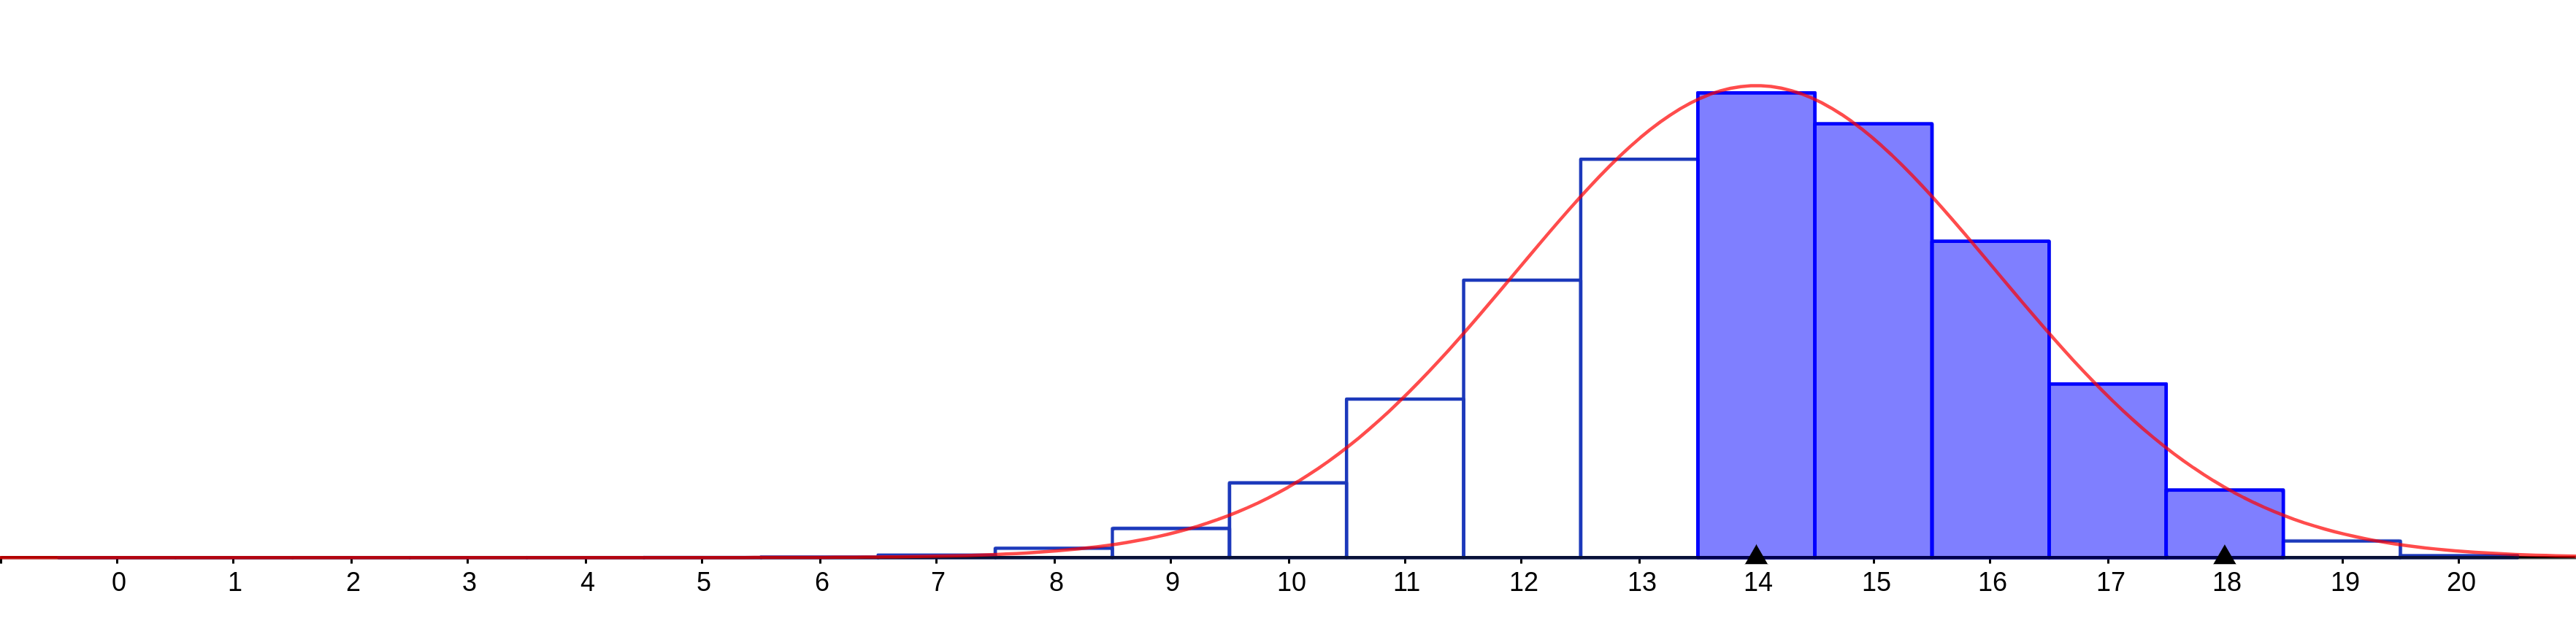
\includegraphics[width=0.5\linewidth]{pics/g2-2} 
		\centering
	\end{figure}\noindent
	Por otro lado, en \texttt{R}, $P(X\leq 10)$ es:
	\begin{lstlisting}[language=R]
> pbinom(10, 20, 0.7, lower.tail = TRUE)
[1] 0.0479619
	\end{lstlisting}
	y $P(14 \leq X \leq 18)$:
	\begin{lstlisting}[language=R]
> sum(dbinom(14:18, 20, 0.7))
[1] 0.6003726
	\end{lstlisting}
\end{sol}
\begin{ejer}[0,5]
	 Para la distribución Binomial $(20, \theta = 0.2)$, $P(X \leq 4)$.
\end{ejer}
\begin{sol}
	Por un lado, con los parámetros $n=20$ y $p=0.2$, \texttt{Geogebra} da una $P(X\leq 4) = 0.6296$ con el siguiente gráfico:
		\begin{figure}[H]
		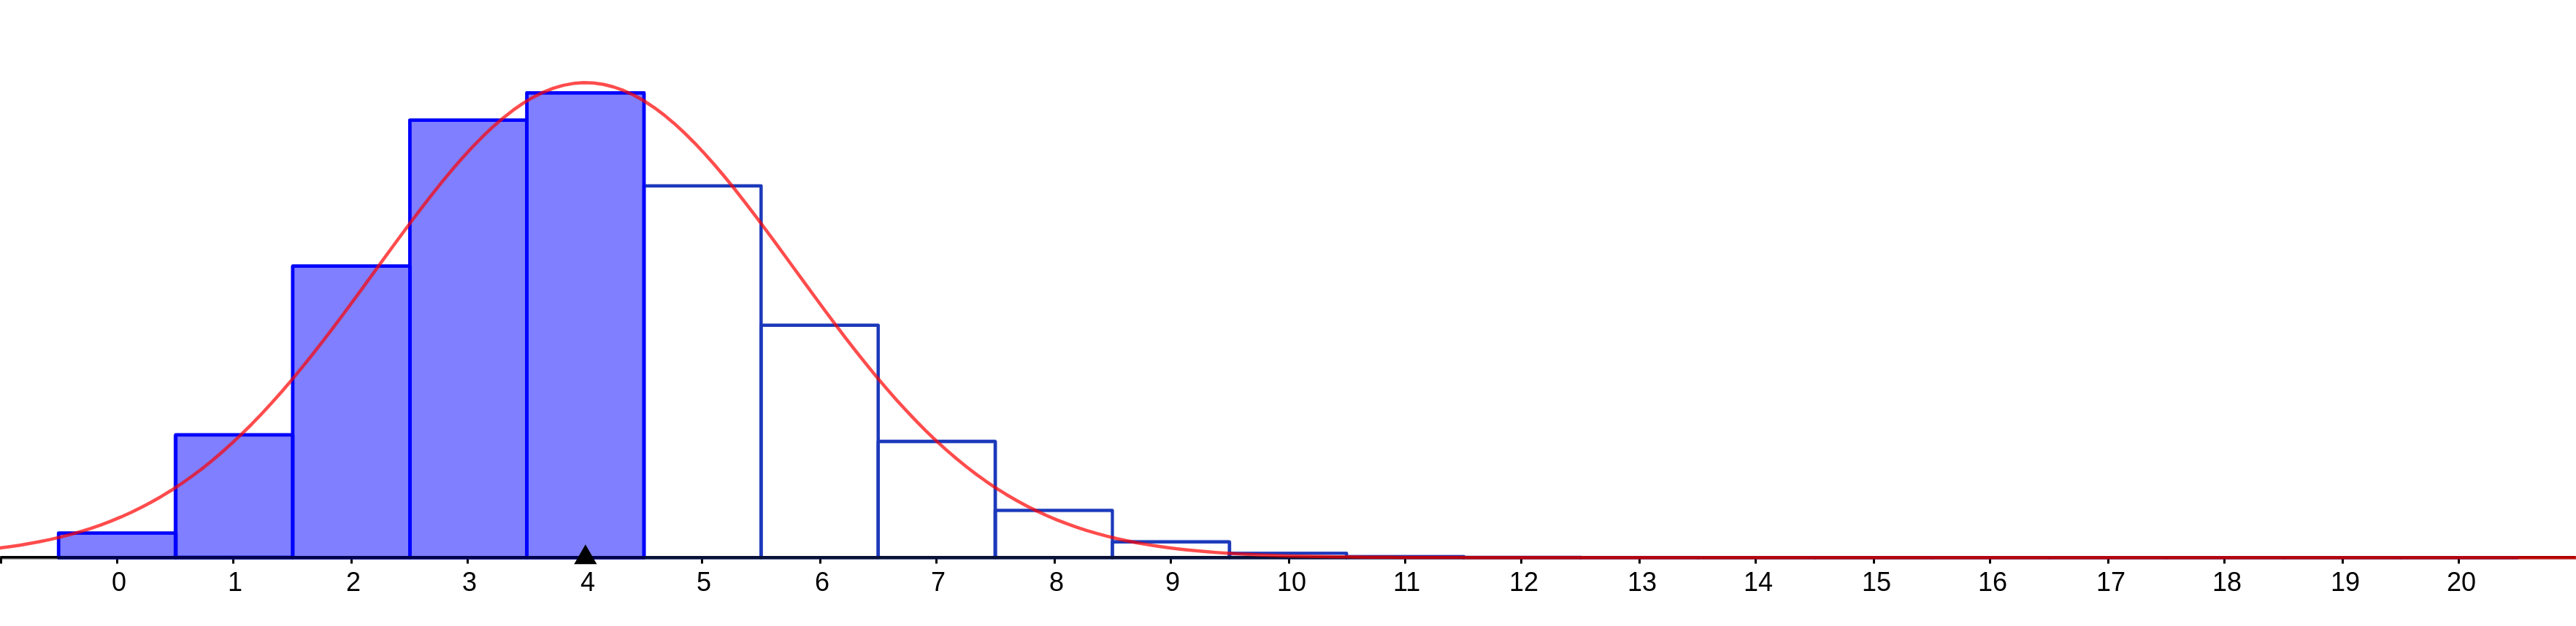
\includegraphics[width=0.5\linewidth]{pics/g3}
		\centering
		\end{figure}\noindent
	Por otro lado, en \texttt{R}, $P(X\leq 4)$ es:
	\begin{lstlisting}[language=R]
> pbinom(4, 20, 0.2, lower.tail = TRUE)
[1] 0.6296483
	\end{lstlisting}
\end{sol}
\begin{ejer}[0,5]
	Para la distribución Binomial $(30, \theta = 0.1)$, $P(X \leq 4)$.	
\end{ejer}
\begin{sol}
	Por un lado, con los parámetros $n=30$ y $p=0.1$, \texttt{Geogebra} da una $P(X\geq 4) = 0.3526$ con el siguiente gráfico:
	\begin{figure}[H]
	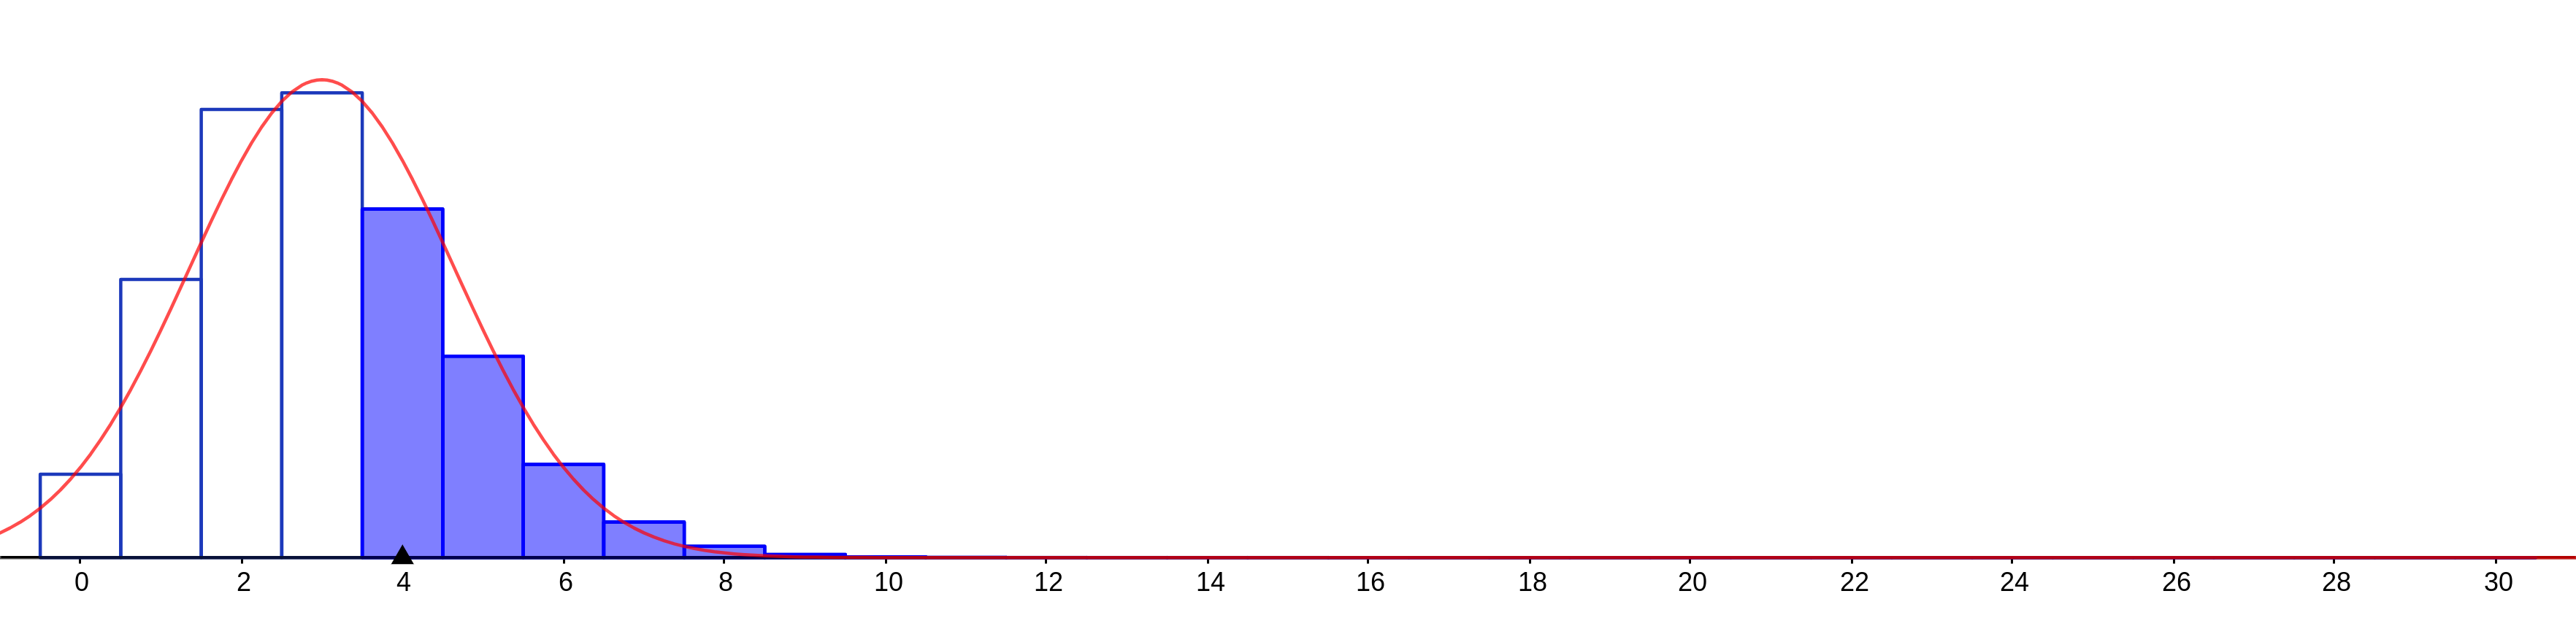
\includegraphics[width=0.5\linewidth]{pics/g4}
	\centering
	\end{figure}\noindent
	Por otro lado, en \texttt{R}, $P(X\geq 4)$ es:
	\begin{lstlisting}[language=R]
> pbinom(3, 30, 0.1, lower.tail = FALSE)
[1] 0.3525608
	\end{lstlisting}
\end{sol}
\begin{ejer}[1]
	 Para la distribución Binomial $(30, \theta = 0.6)$, $P(X \leq 18)$ y $P(X \geq 20)$.
\end{ejer}
\begin{sol}
	Por un lado, con los parámetros $n=30$ y $p=0.6$, \texttt{Geogebra} da una $P(X\leq 18) = 0.5689$ con el siguiente gráfico:
	\begin{figure}[H]
	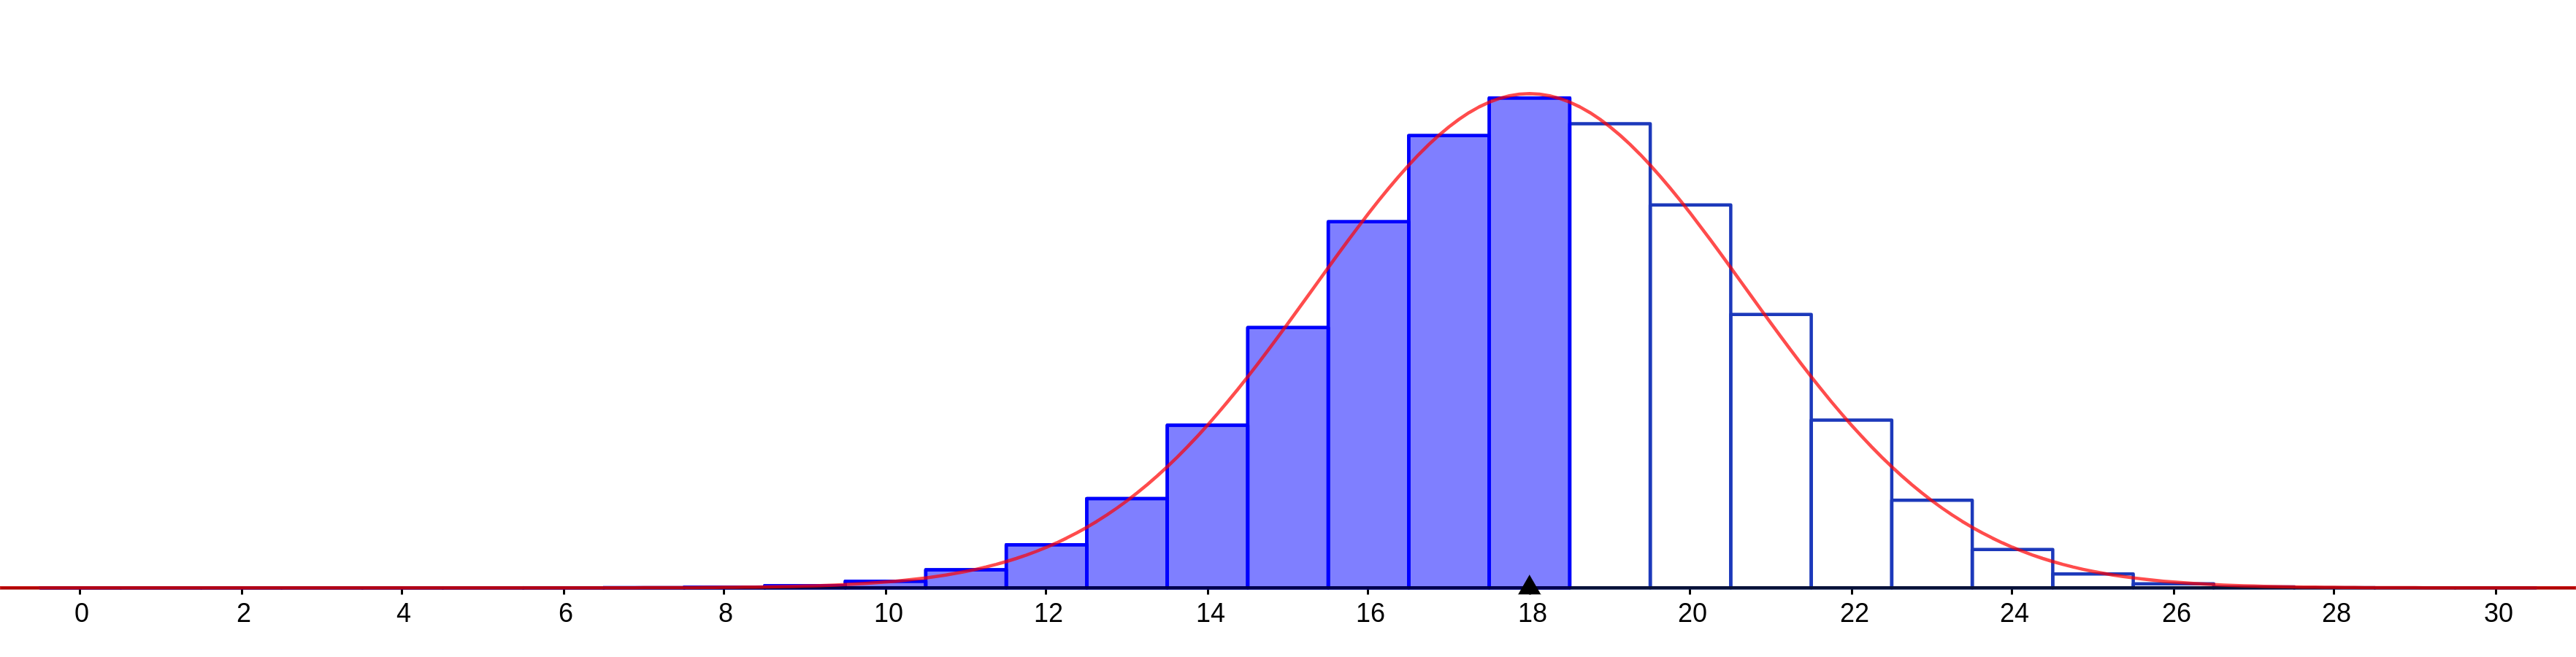
\includegraphics[width=0.5\linewidth]{pics/g5-1}
	\centering
	\end{figure}\noindent
	y $P(X \geq 20) = 0.2915$ con el gráfico:
	\begin{figure}[H]
	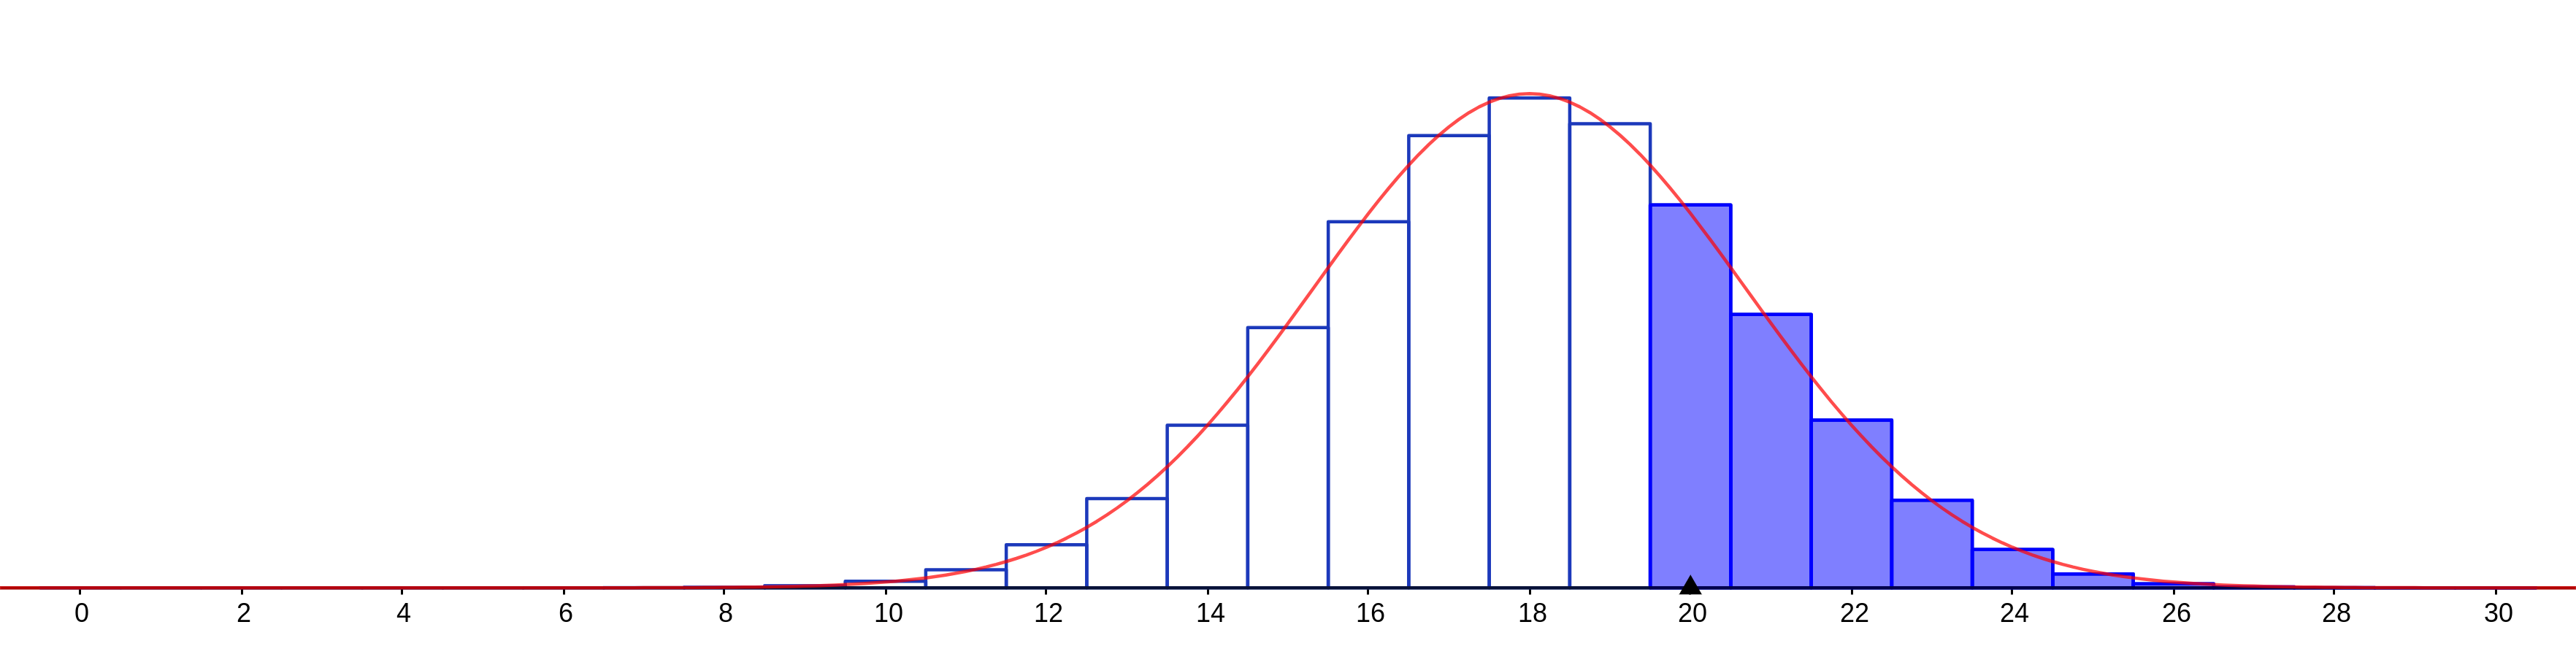
\includegraphics[width=0.5\linewidth]{pics/g5-2}
	\centering
	\end{figure}\noindent
	Por otro lado, en \texttt{R}, $P(X\leq 18)$ es:
	\begin{lstlisting}[language=R]
> pbinom(18, 30, 0.6, lower.tail = TRUE)
[1] 0.5689095
	\end{lstlisting}
	y $P(X \geq 20)$:
	\begin{lstlisting}[language=R]
> pbinom(19, 30, 0.6, lower.tail = FALSE)
[1] 0.2914719
	\end{lstlisting}
\end{sol}

\subsection{Distribución geometrica}
\begin{ejer}[0,25]
	 Para la distribución geométrica (Pascal) $(1, \theta = 0.36)$, $P(X \leq 4)$.
\end{ejer}
\begin{sol}
	Por un lado, con los parámetros $n=1$ y $p=0.36$, \texttt{Geogebra} da una $P(X\leq 4) = 0.8926$ con el siguiente gráfico:
	\begin{figure}[H]
	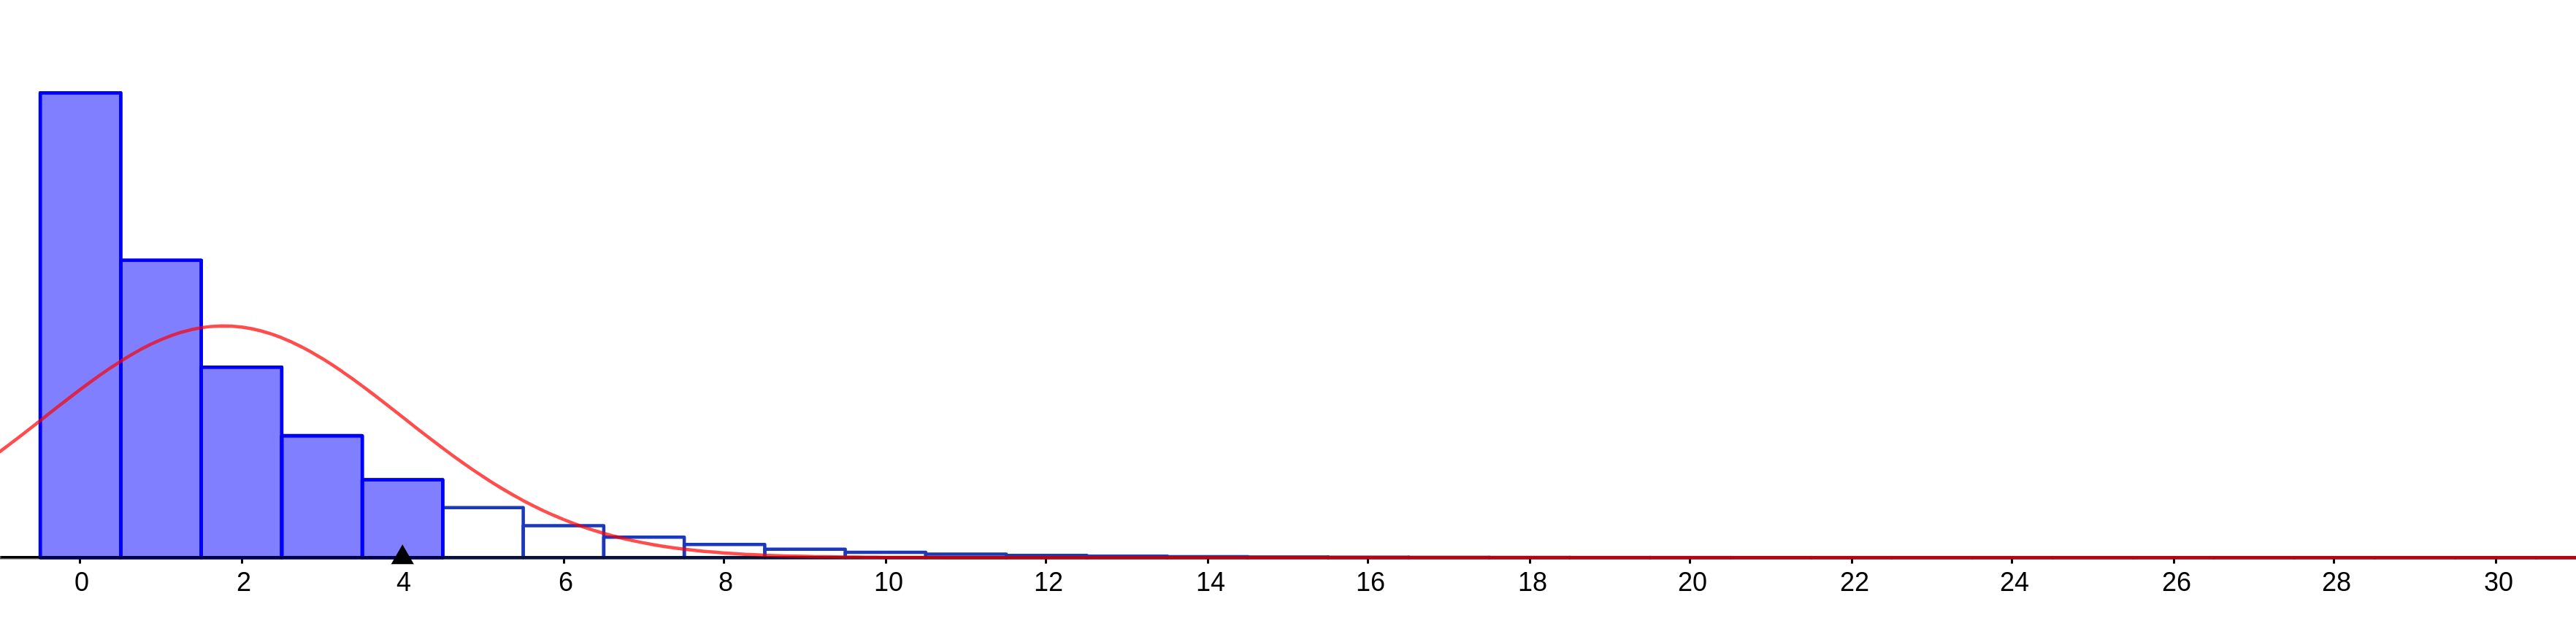
\includegraphics[width=0.5\linewidth]{pics/g6}
	\centering
	\end{figure}\noindent
	Por otro lado, en \texttt{R}, $P(X\leq 4)$ es:
	\begin{lstlisting}[language=R]
> pgeom(4, 0.36, lower.tail = TRUE)
[1] 0.8926258
	\end{lstlisting}
\end{sol}
\begin{ejer}[0,25]
	 Para la distribución geométrica (Pascal) $(1, \theta = 0.72)$, $P(X\geq 2)$.
\end{ejer}
\begin{sol}
	Por un lado, con los parámetros $n=1$ y $p=0.72$, \texttt{Geogebra} da una $P(X\geq 2) = 0.0784$ con el siguiente gráfico:
	\begin{figure}[H]
	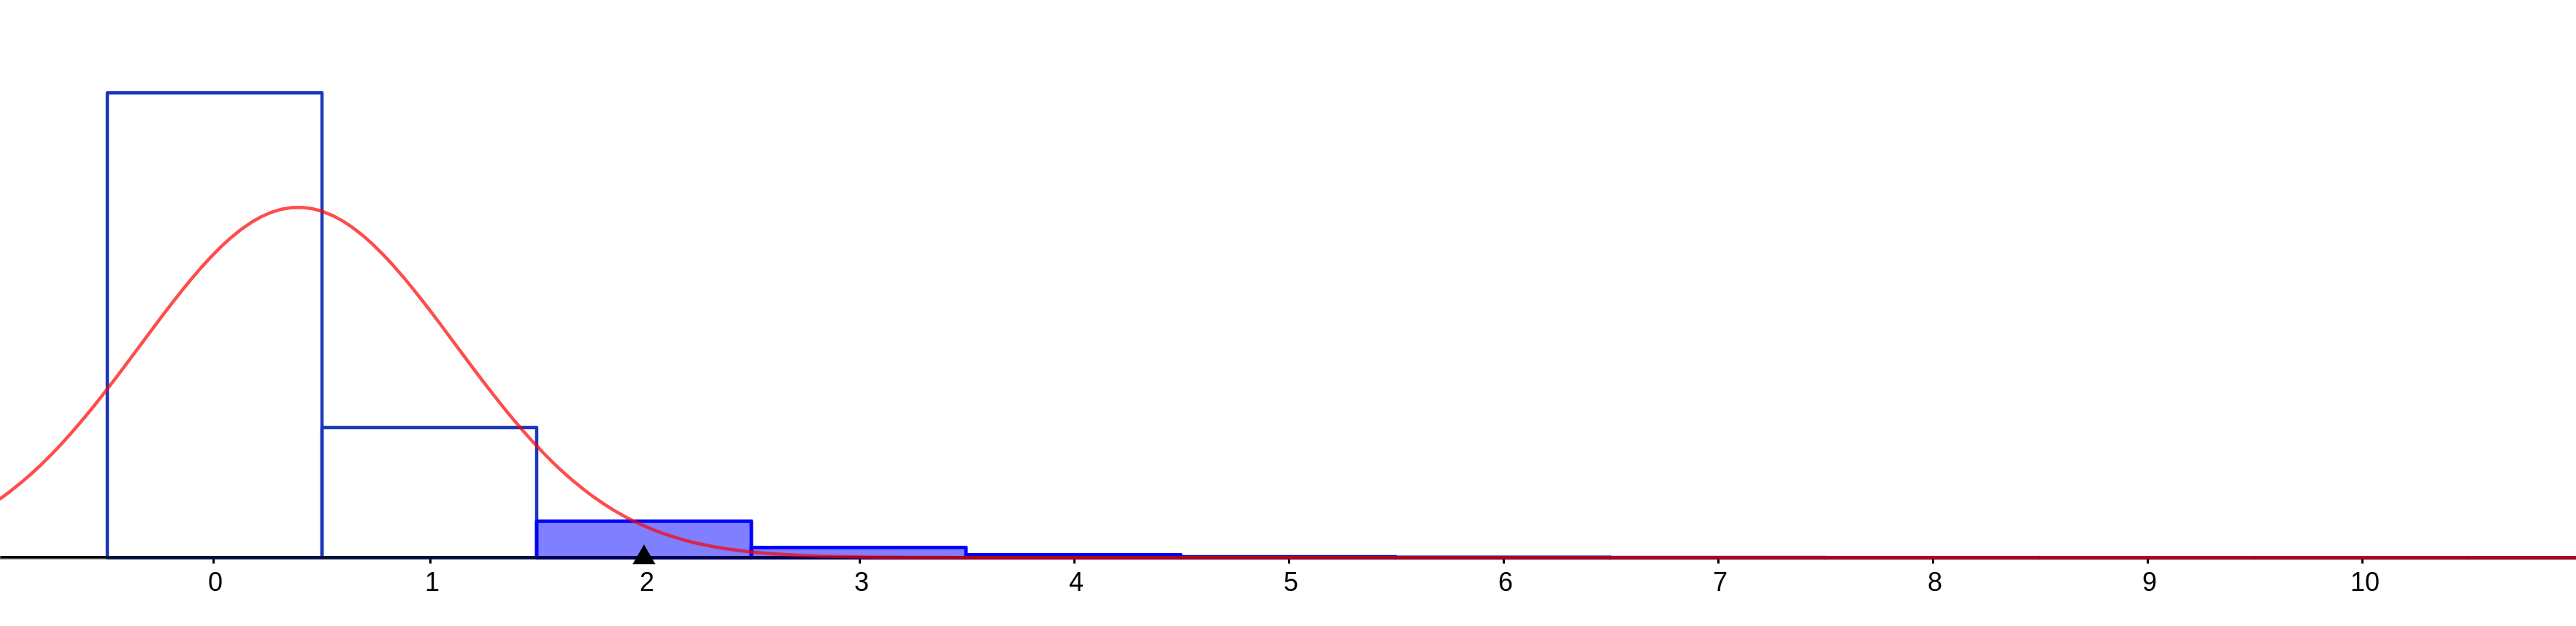
\includegraphics[width=0.5\linewidth]{pics/g7}
	\centering
	\end{figure}\noindent
	Por otro lado, en \texttt{R}, $P(X\geq 2)$ es:
	\begin{lstlisting}[language=R]
> pgeom(1, 0.72, lower.tail = FALSE)
[1] 0.0784
	\end{lstlisting}
\end{sol}

\subsection{Distribución binomial negativa}
\begin{ejer}[1]
	 Para la distribución Binomial negativa (Pascal) $(2, \theta = 0.2)$, $P(X \leq 3)$ y $P(X\geq 15)$.
\end{ejer}
\begin{sol}
	Por un lado, con los parámetros $n=2$ y $p=0.2$, \texttt{Geogebra} da una $P(X\leq 3) = 0.2627$ con el siguiente gráfico:
	\begin{figure}[H]
	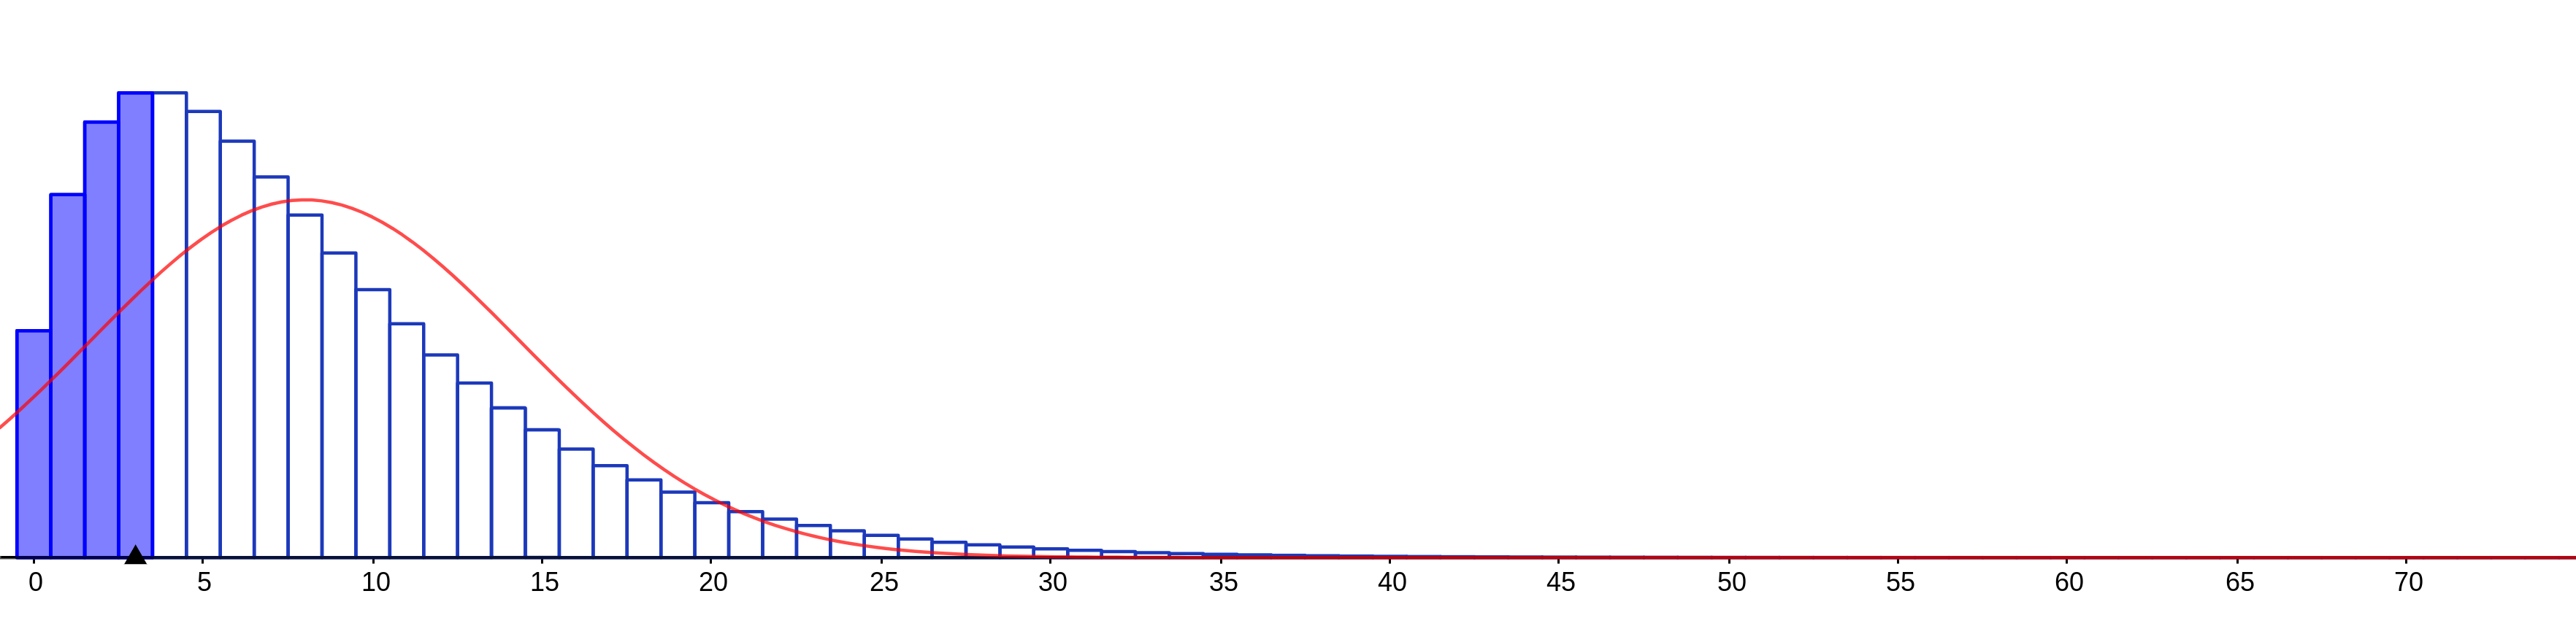
\includegraphics[width=0.5\linewidth]{pics/g8}
	\centering
	\end{figure}\noindent
	y $P(X\geq 15) = 0.1407$ con el gráfico:
	\begin{figure}[H]
	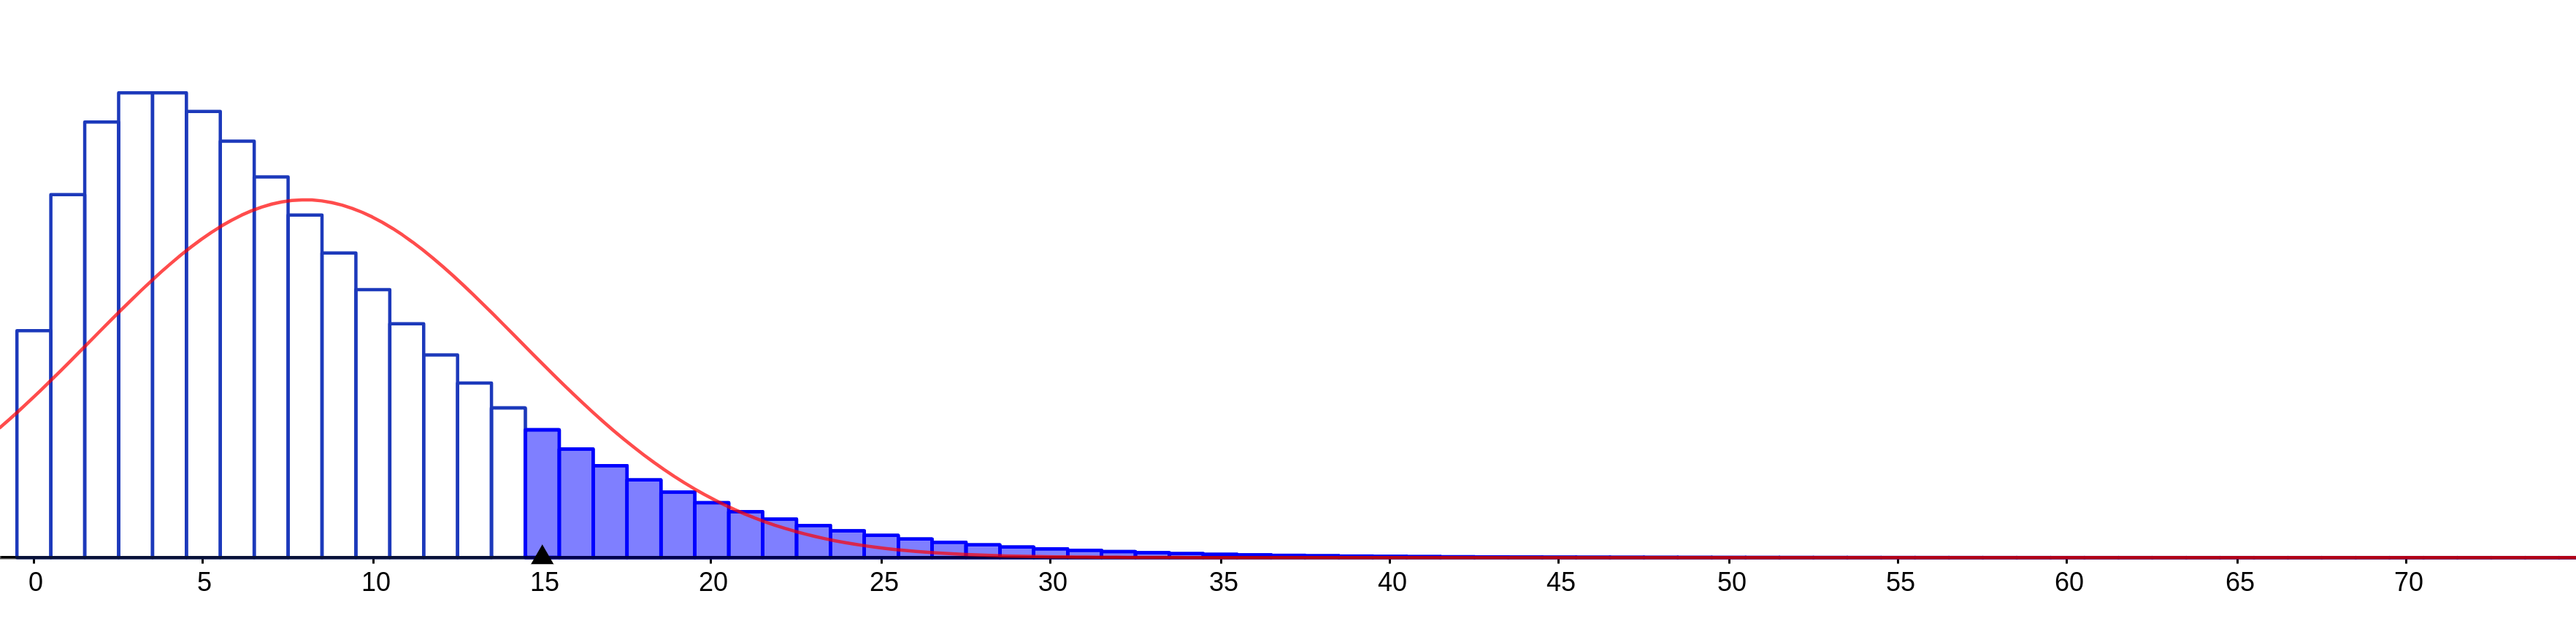
\includegraphics[width=0.5\linewidth]{pics/g8-2}
	\centering
	\end{figure}\noindent
	Por otro lado, en \texttt{R}, $P(X\leq 3)$ es:
	\begin{lstlisting}[language=R]
> pnbinom(3, 2, 0.2, lower.tail = TRUE)
[1] 0.26272
	\end{lstlisting}
	y $P(X\geq 15)$:
	\begin{lstlisting}[language=R]
> pnbinom(14, 2, 0.2, lower.tail = FALSE)
[1] 0.1407375
	\end{lstlisting}
\end{sol}
\begin{ejer}
		 Para la distribución Binomial negativa (Pascal) $(8, \theta = 0.6)$, $P(X \leq 4)$ y $P(X\geq 8)$.
\end{ejer}
\begin{sol}
	Por un lado, con los parámetros $n=8$ y $p=0.6$, \texttt{Geogebra} da una $P(X\leq 4) = 0.4382$ con el siguiente gráfico:
	\begin{figure}[H]
	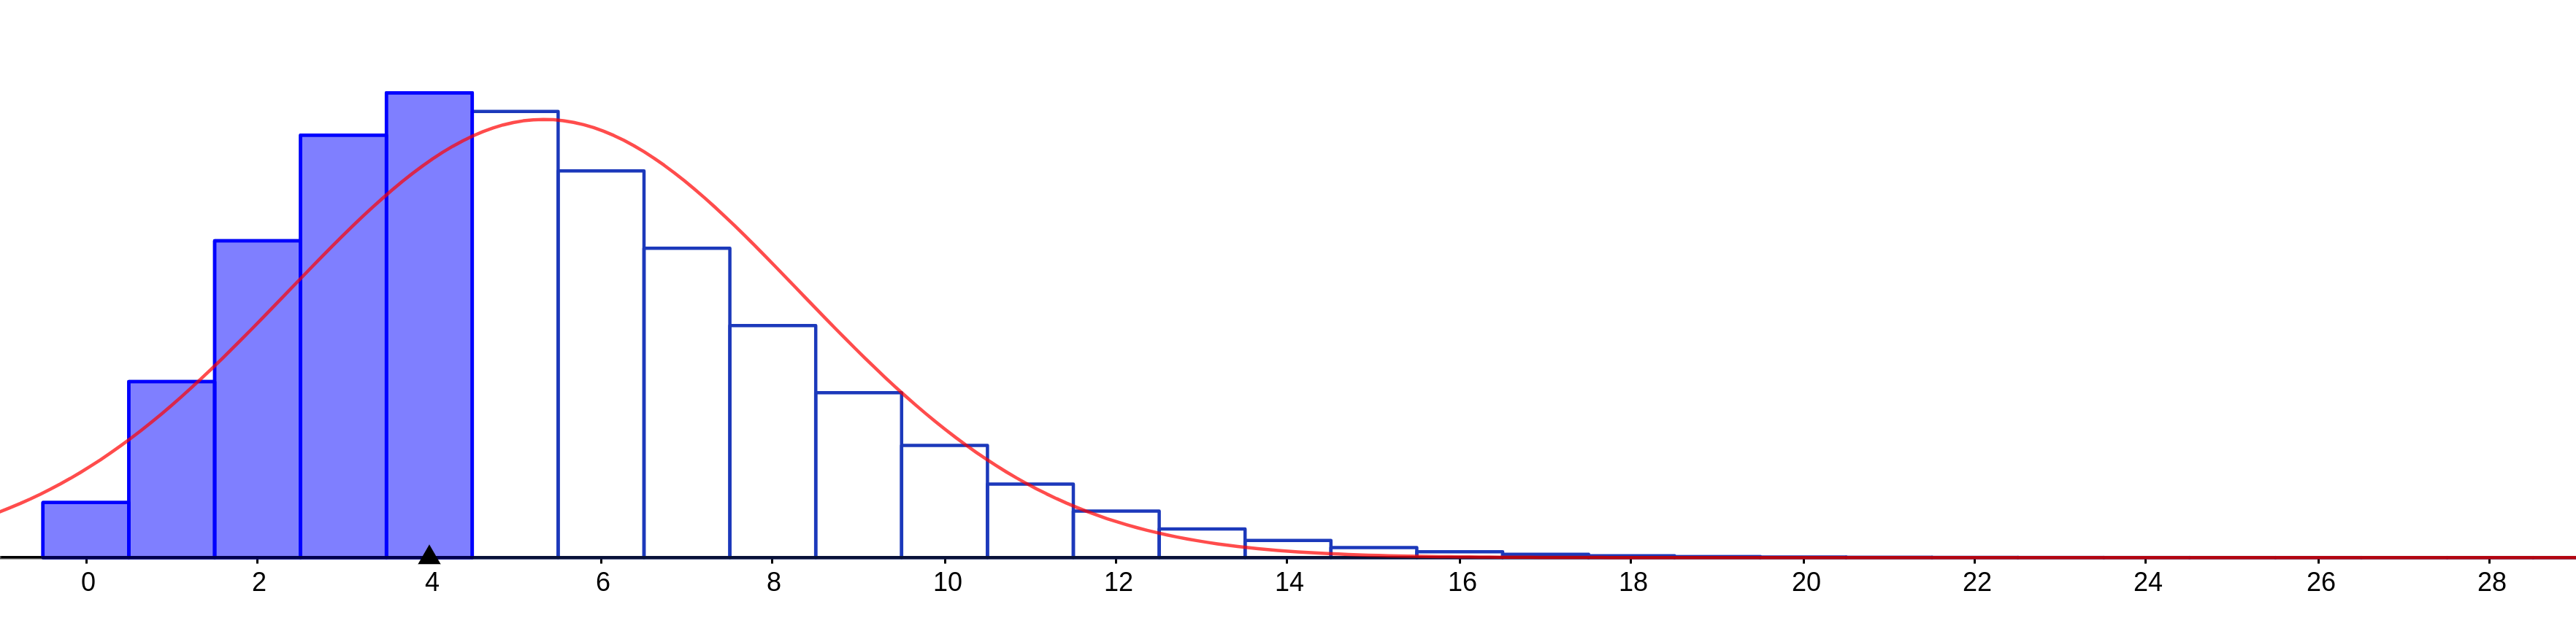
\includegraphics[width=0.5\linewidth]{pics/g9-1}
	\centering
	\end{figure}\noindent
	y $P(X\geq 8) = 0.2131$ con el gráfico:
	\begin{figure}[H]
	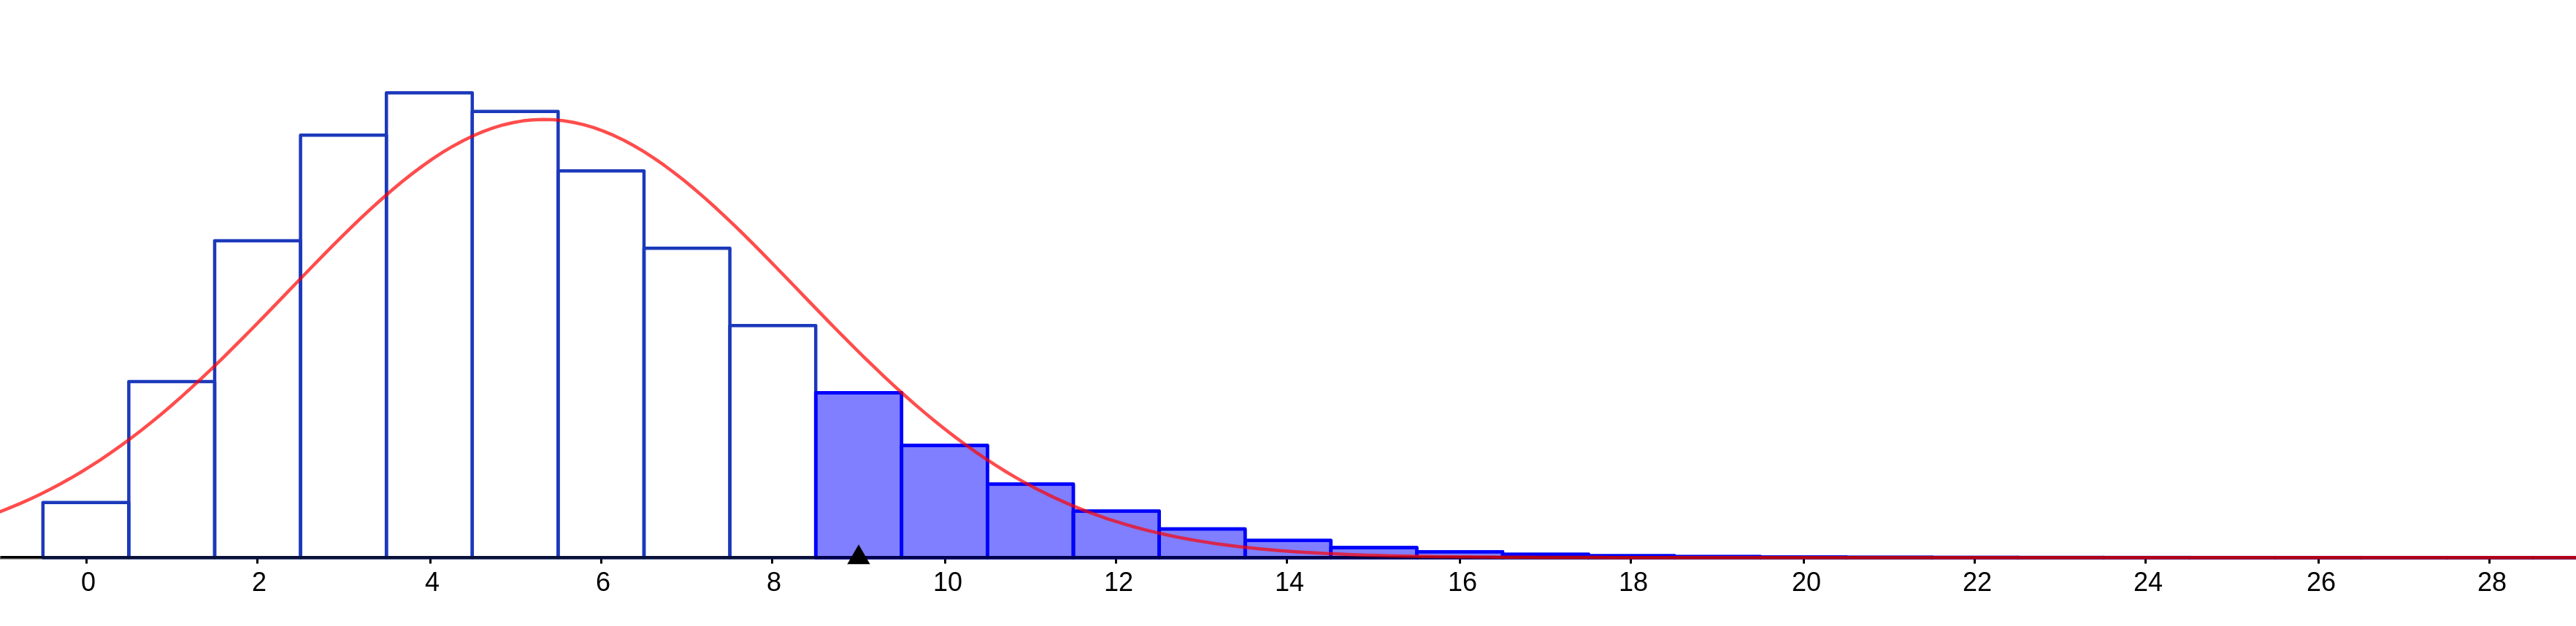
\includegraphics[width=0.5\linewidth]{pics/g9-2}
	\centering
	\end{figure}\noindent
	Por otro lado, con \texttt{R} tenemos que $P(X\leq 4)$:
	\begin{lstlisting}[language=R]
> pnbinom(4, 8, 0.6, lower.tail = TRUE)
[1] 0.4381782
	\end{lstlisting}
	y $P(X\geq 8)$:
	\begin{lstlisting}[language=R]
> pnbinom(7, 8, 0.6, lower.tail = FALSE)
[1] 0.2131032
	\end{lstlisting}
\end{sol}

\subsection{Distribución Poission}
\begin{ejer}[1]
	 Para la distribución Poisson $(\lambda = 14)$, $P(X\leq 10)$ y $P(X\geq 16)$.
\end{ejer}
\begin{sol}
	Por un lado, con el parámetro $\mu=14$, \texttt{Geogebra} da una $P(X\leq 10) = 0.1757$ con el siguiente gráfico:
	\begin{figure}[H]
	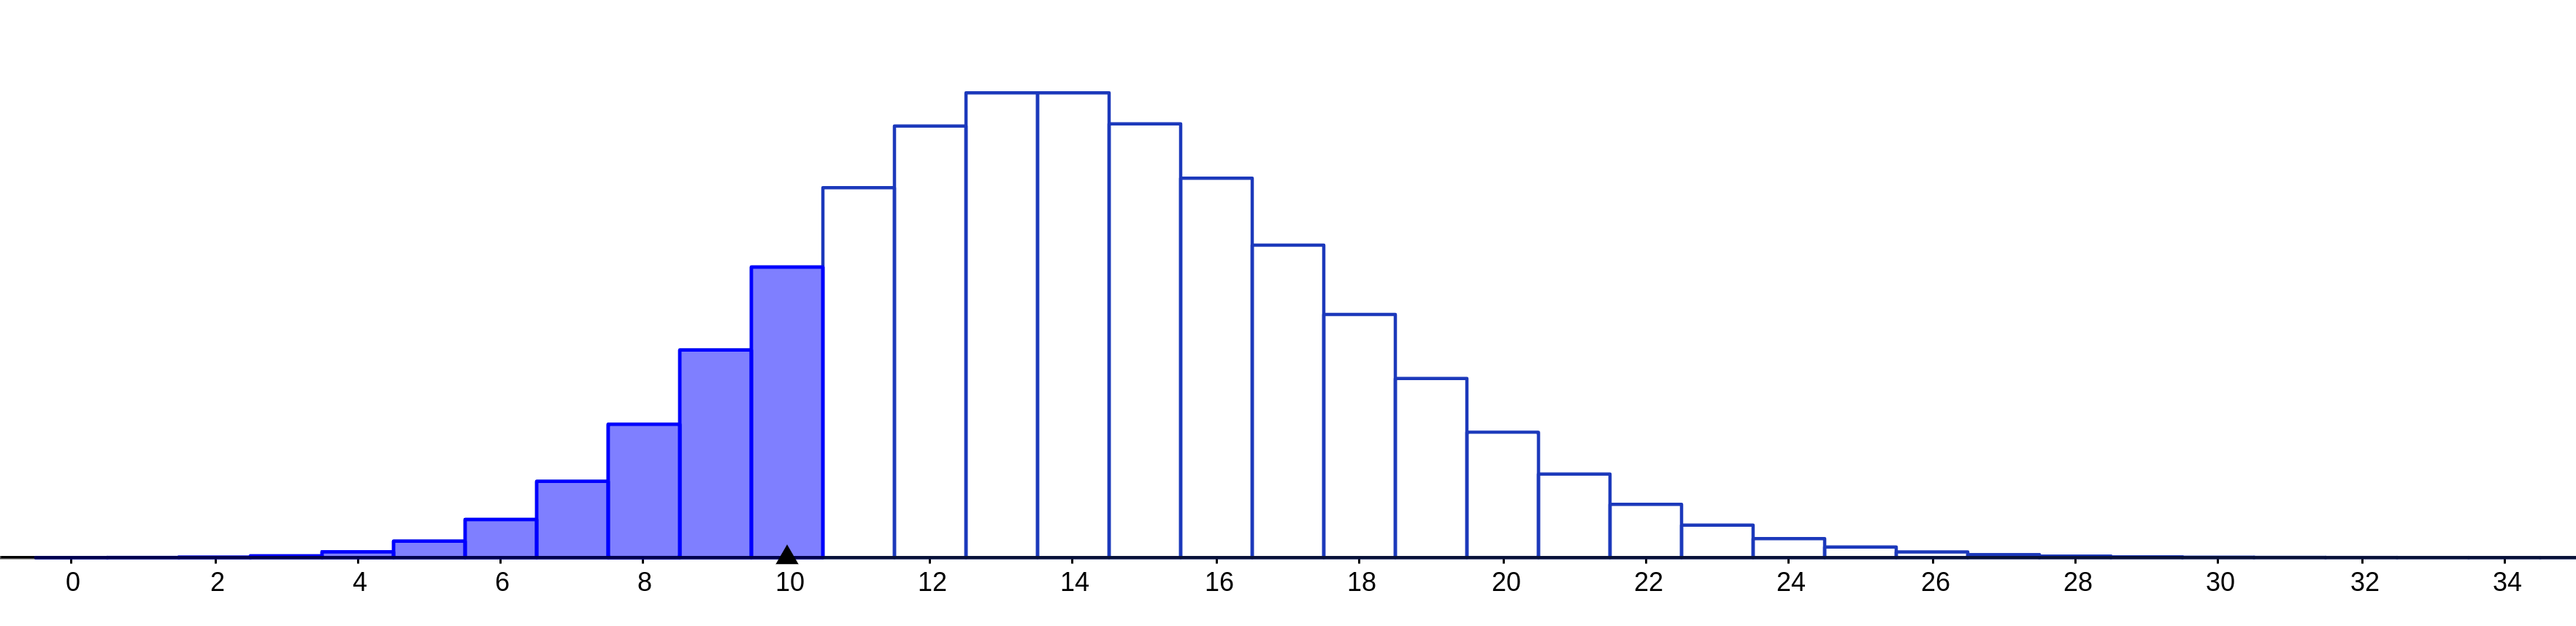
\includegraphics[width=0.5\linewidth]{pics/g10-1}
	\centering
	\end{figure}\noindent
	y $P(X\geq 16) = 0.3306$ con el gráfico:
	\begin{figure}[H]
	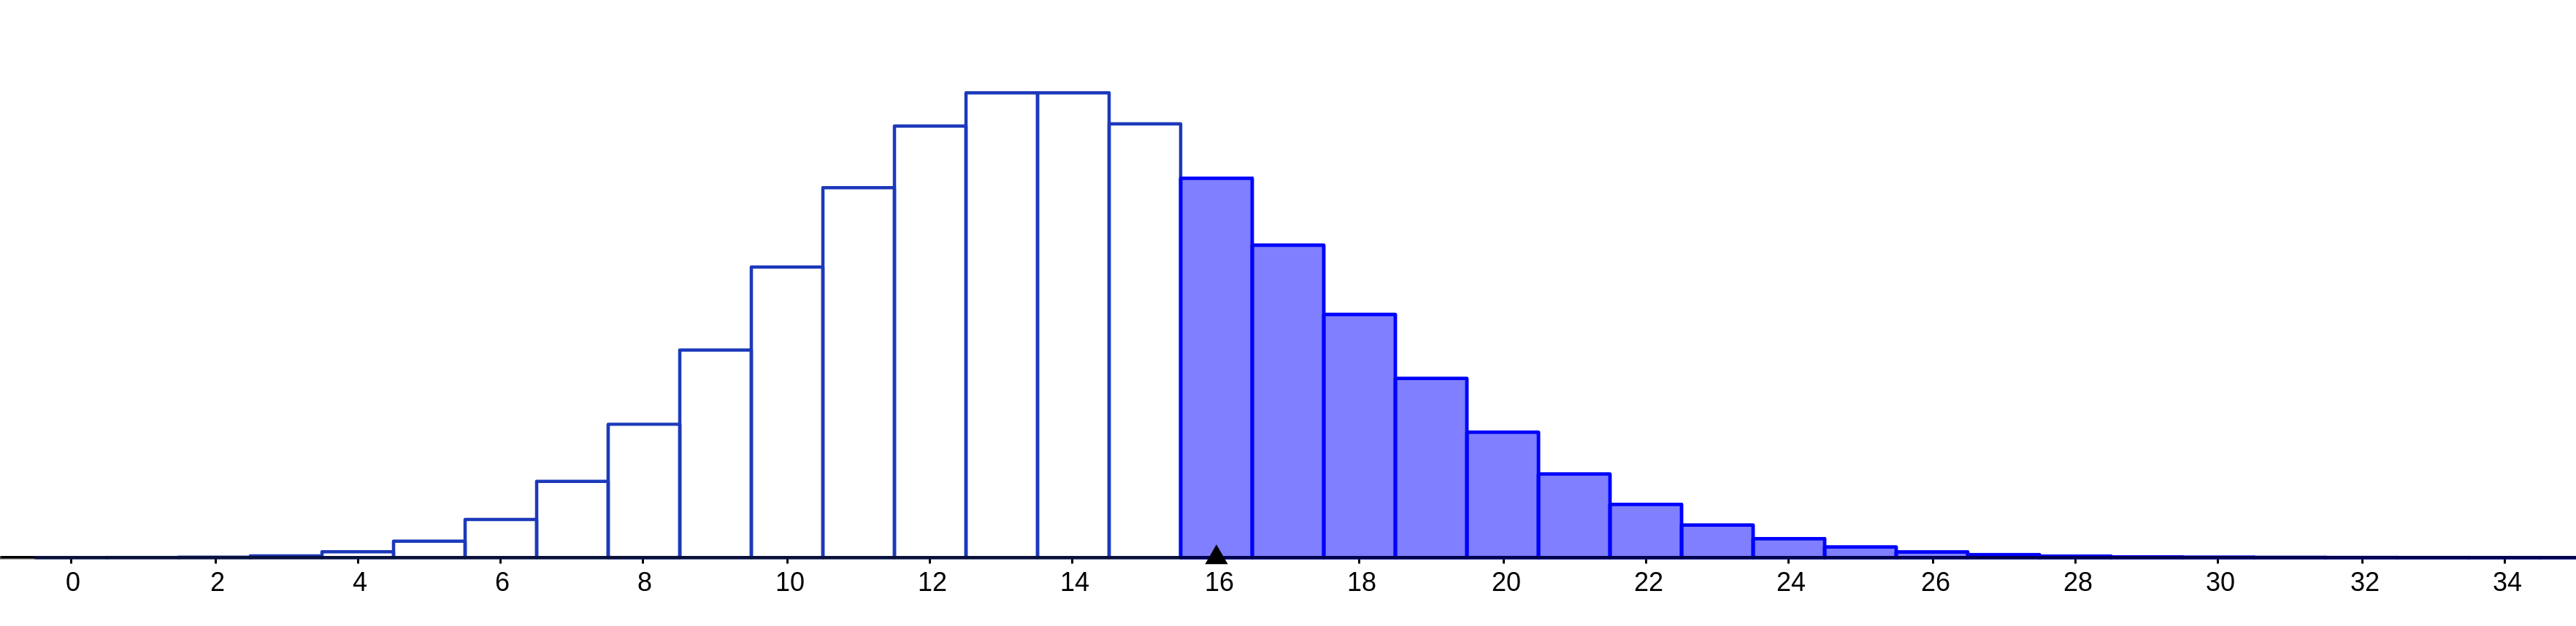
\includegraphics[width=0.5\linewidth]{pics/g10-2}
	\centering
	\end{figure}\noindent
	Por otro lado, en \texttt{R}, $P(X\leq 10)$ es:
	\begin{lstlisting}[language=R]
> ppois(10, 14, lower.tail = TRUE)
[1] 0.1756812
	\end{lstlisting}
	y $P(X\geq 16)$:
		\begin{lstlisting}[language=R]
> ppois(15, 14, lower.tail = FALSE)
[1] 0.3306401
	\end{lstlisting}
\end{sol}
\begin{ejer}[1]
	Para la distribución Poisson $(\lambda = 34)$, $P(X \leq 40)$ y $P(X\geq 28)$.
\end{ejer}
\begin{sol}
	Por un lado, con el parámetro $\mu=34$, \texttt{Geogebra} da una $P(X\leq 40) = 0.8664$ con el siguiente gráfico:
	\begin{figure}[H]
		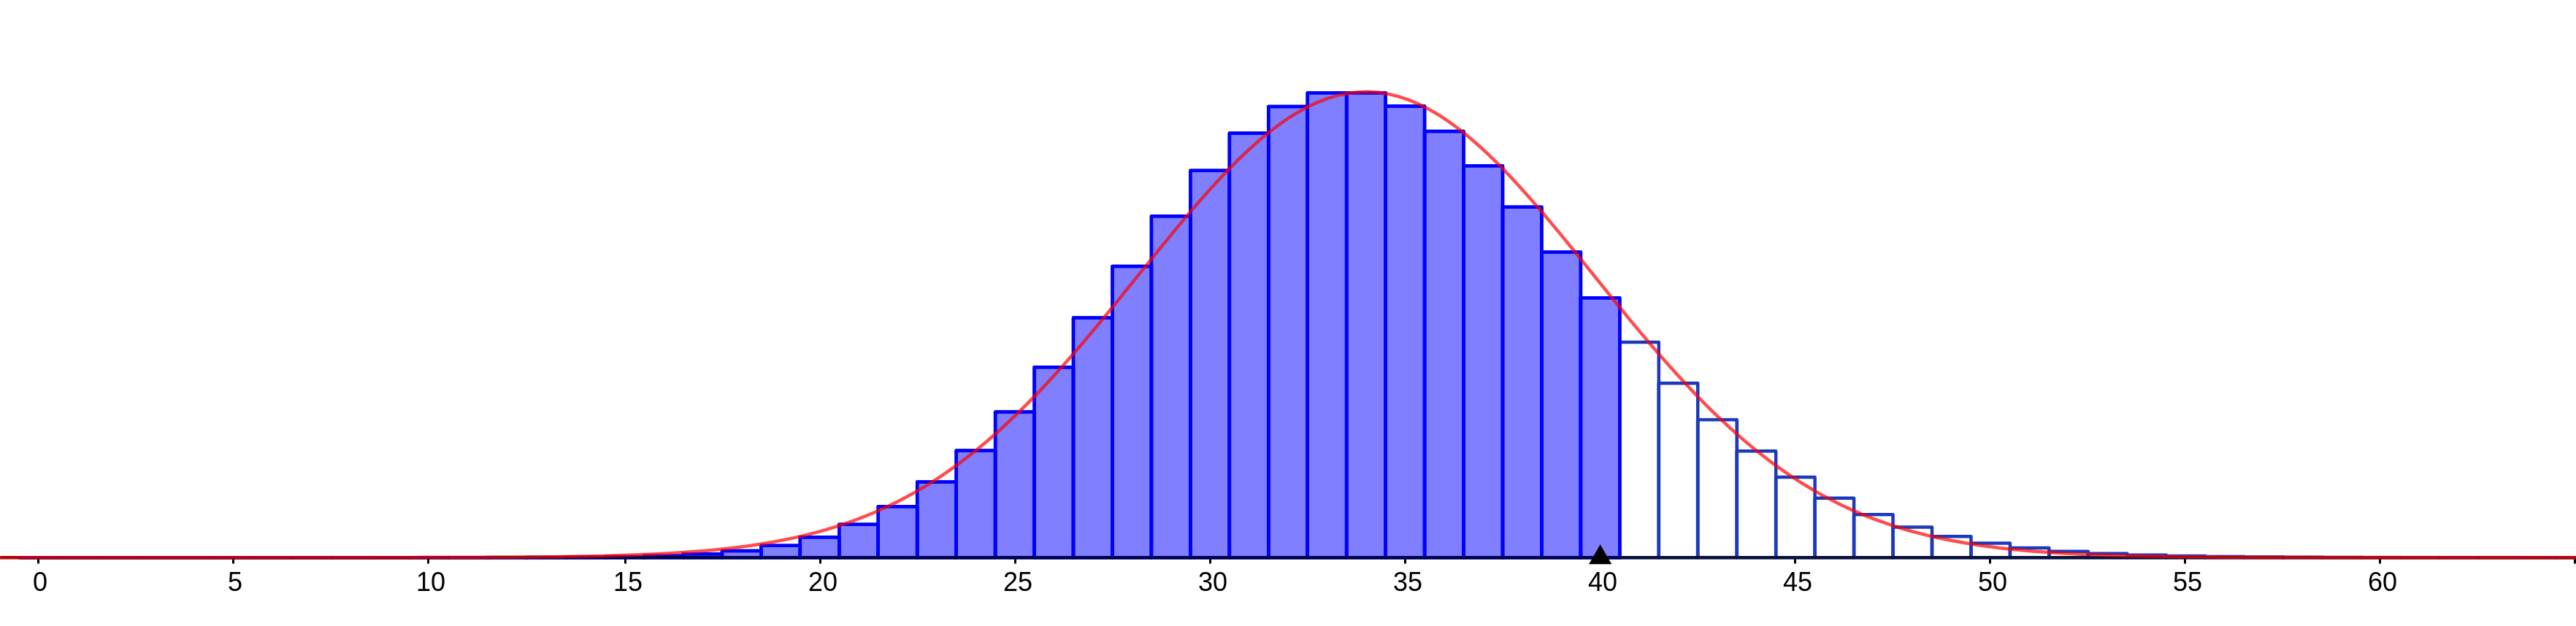
\includegraphics[width=0.5\linewidth]{pics/g11-1}
		\centering
	\end{figure}\noindent
	y $P(X\geq 28) = 0.8694$ con el gráfico:
	\begin{figure}[H]
		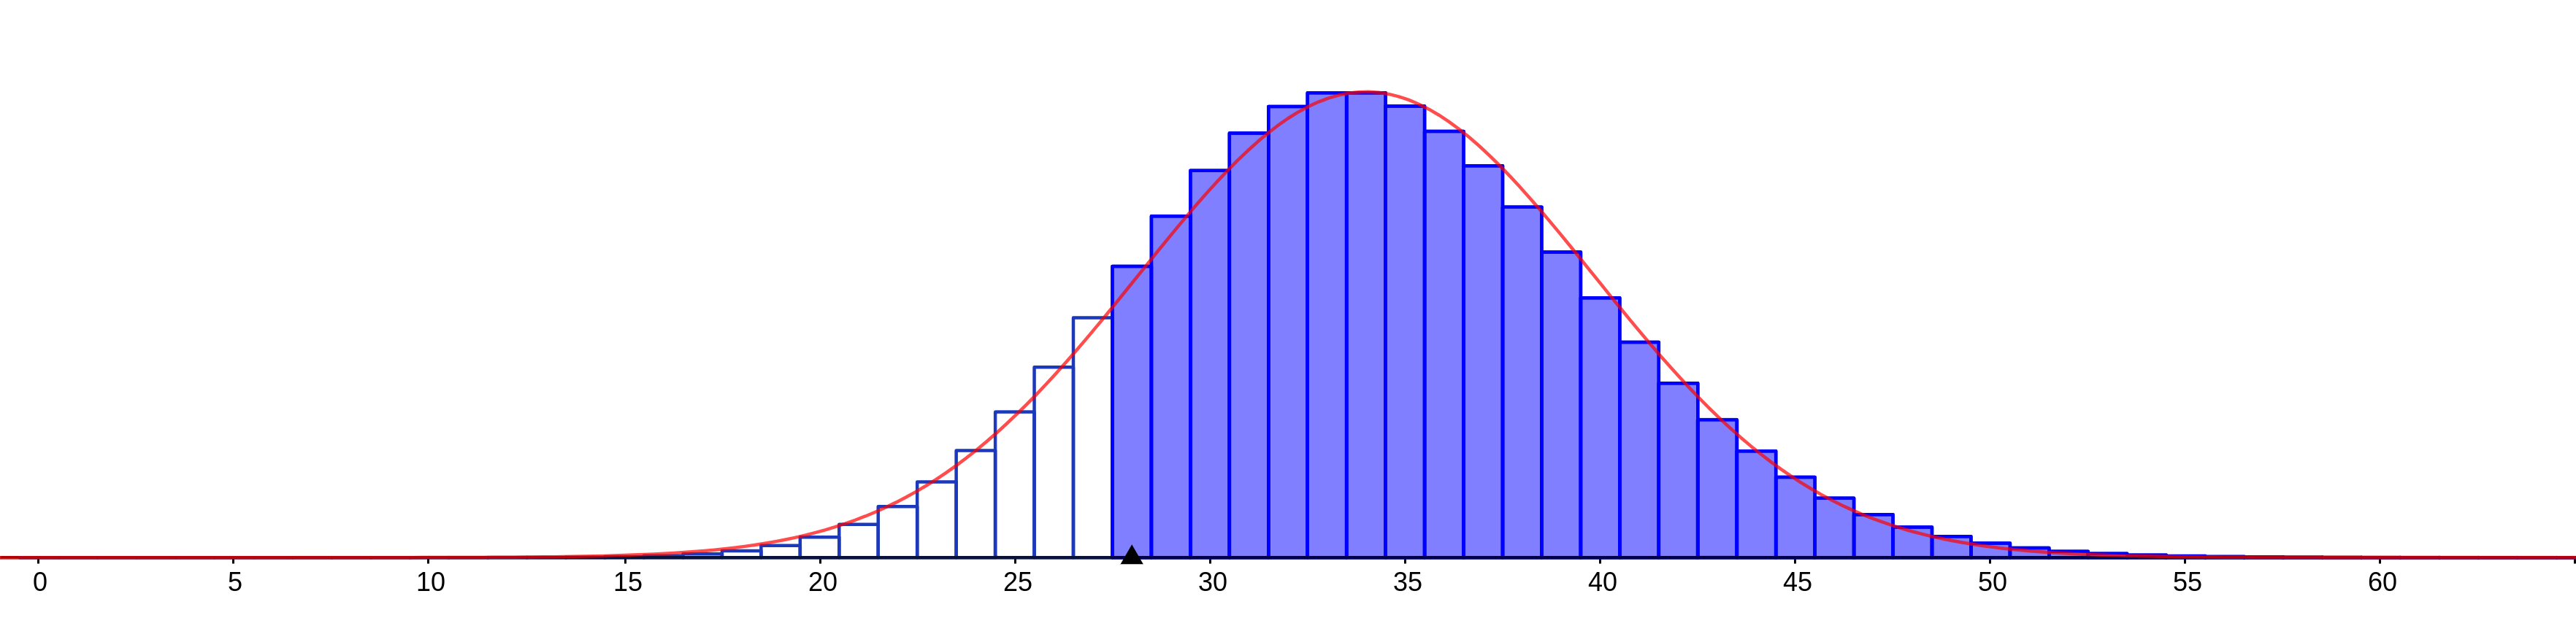
\includegraphics[width=0.5\linewidth]{pics/g11-2}
		\centering
	\end{figure}\noindent
	Por otro lado, en \texttt{R}, $P(X\leq 40)$ es:
	\begin{lstlisting}[language=R]
> ppois(40, 34, lower.tail = TRUE)
[1] 0.8664154
	\end{lstlisting}
	y $P(X\geq 28)$:
	\begin{lstlisting}[language=R]
> ppois(27, 34, lower.tail = FALSE)
[1] 0.8694343
	\end{lstlisting}
\end{sol}

\subsection{Distribución hipergeométrica}
\begin{ejer}
	Para la distribución Hipergeométrica $(600, 140, 20)$, $P(X \leq 5)$ y $P(X \geq 6)$.
\end{ejer}
\begin{sol}
	Por un lado, con los parámetros `$\text{población} = 600$'\;`$n=140$'\;`$\text{muestra} = 20$', \texttt{Geogebra} da una $P(X\leq 5) = 0.6854$ con el siguiente gráfico:
	 \begin{figure}[H]
	 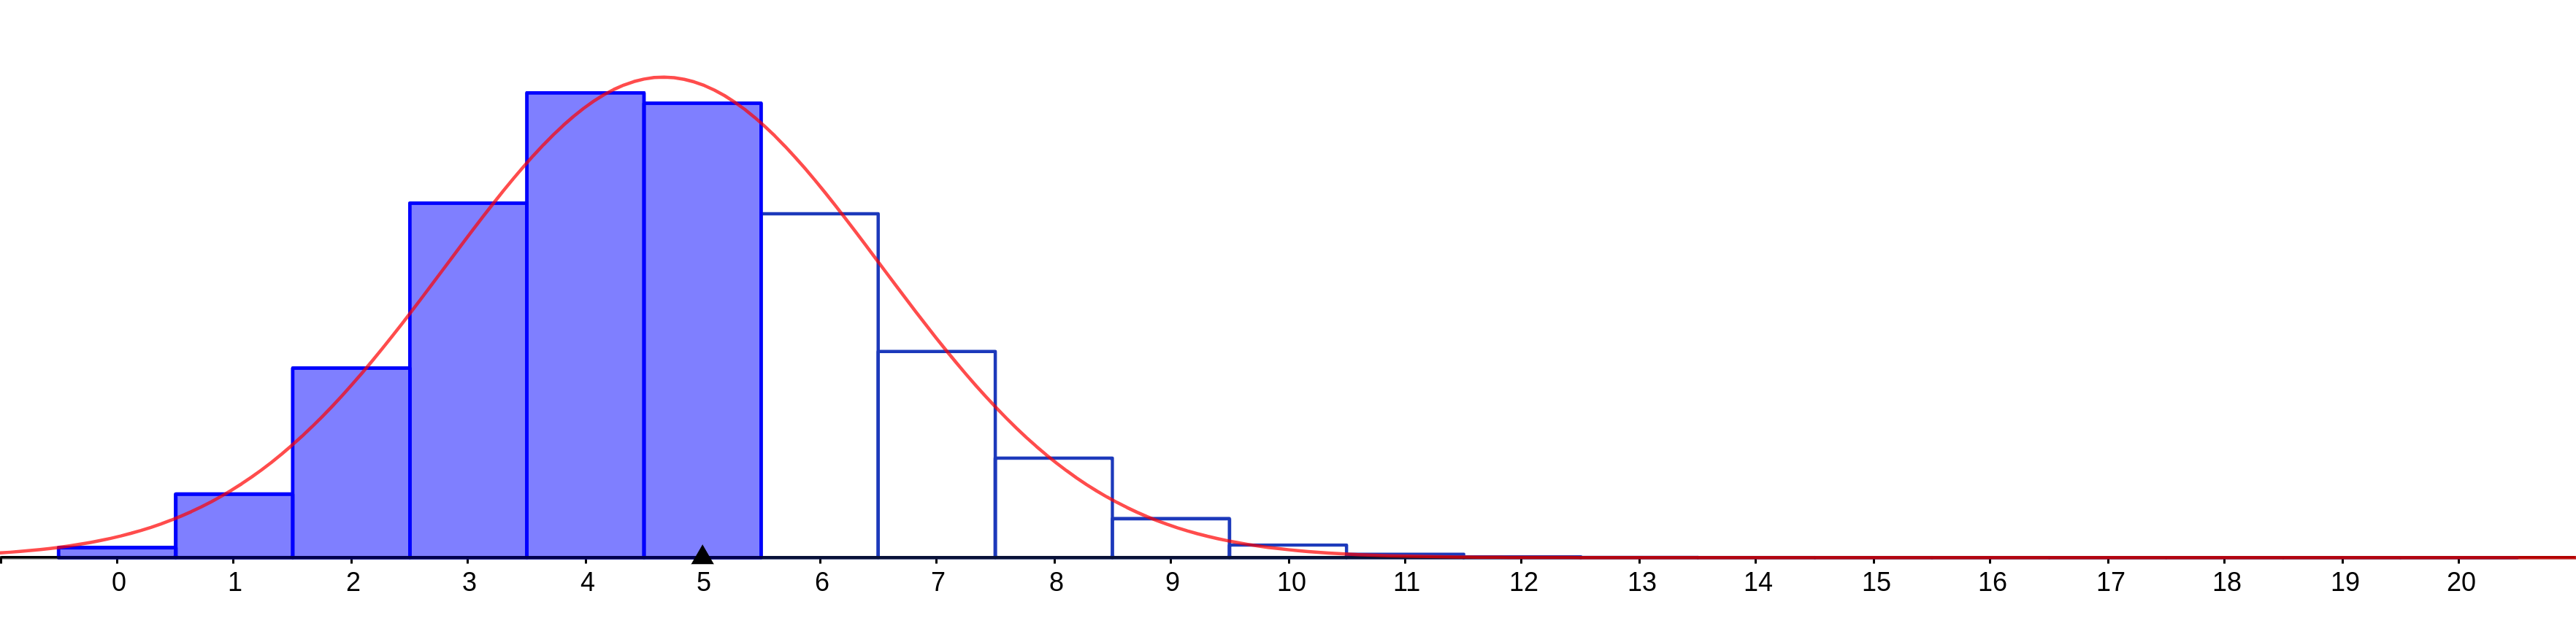
\includegraphics[width=0.5\linewidth]{pics/g12-1}
	 \centering
	 \end{figure}\noindent
 	y una $P(X\geq 6) = 0.3146$  con el gráfico:
 	\begin{figure}[H]
 	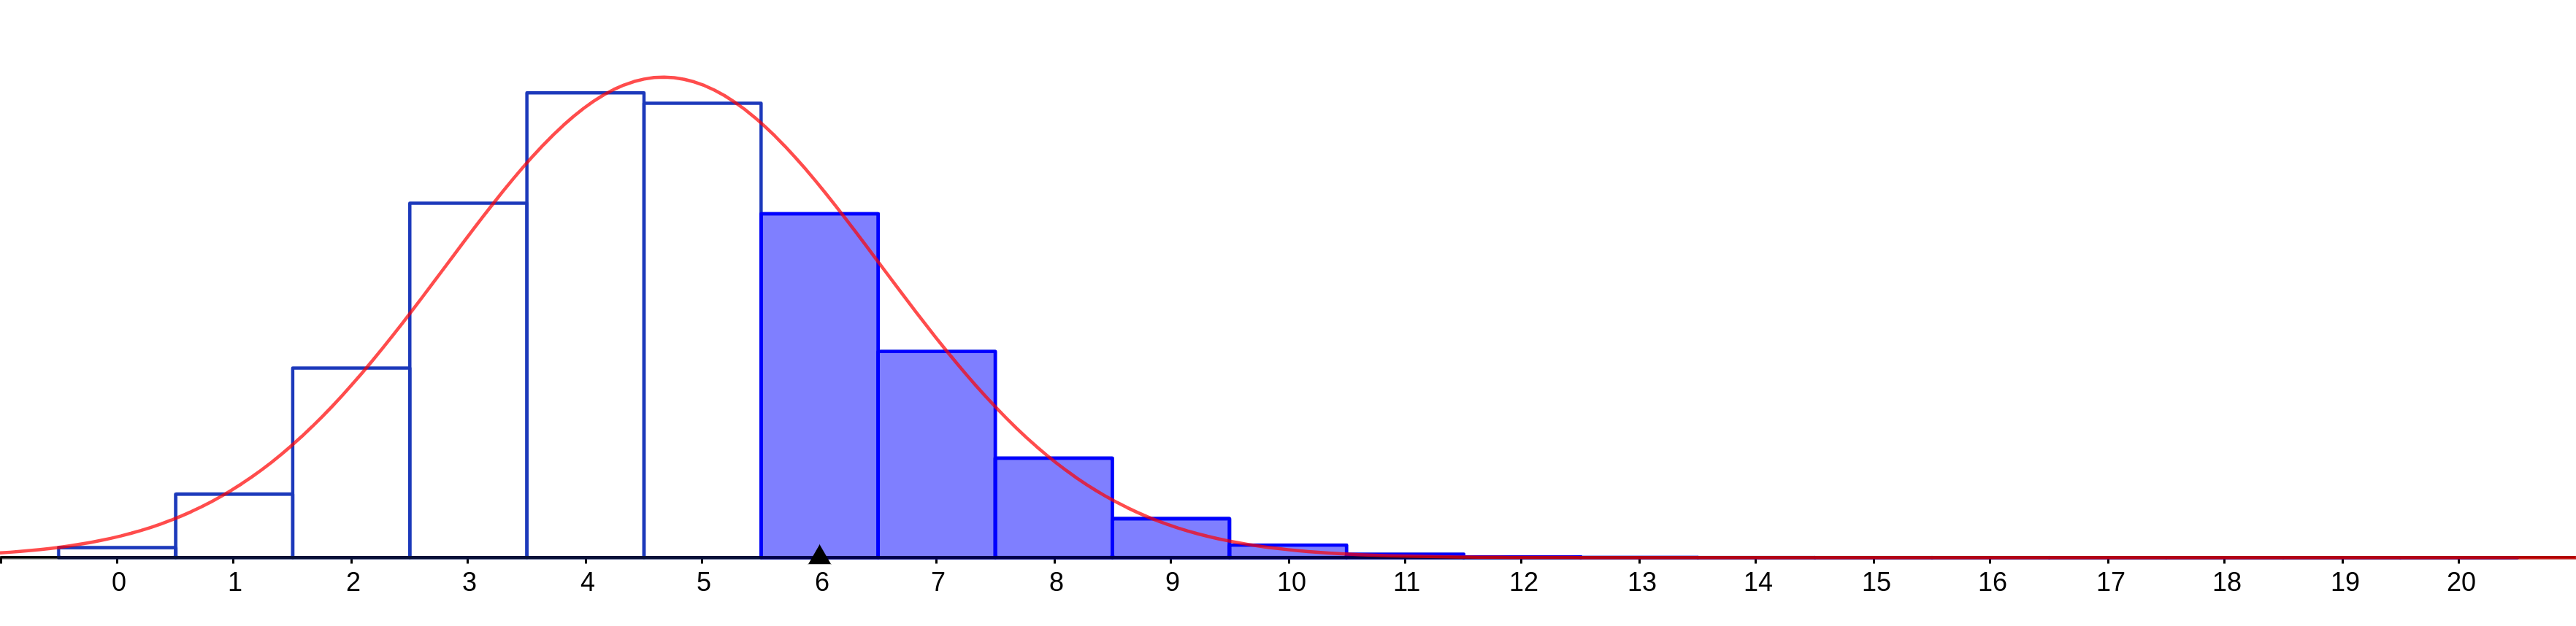
\includegraphics[width=0.5\linewidth]{pics/g12-2}
 	\centering
 	\end{figure}\noindent
 	Por otro lado, en \texttt{R}, $P(X\leq 5)$ es:
 	\begin{lstlisting}[language=R]
> phyper(5, 140, 600-140, 20, lower.tail = TRUE)
[1] 0.6854411
 	\end{lstlisting}
 	y la $P(X\geq 6)$ es:
 	\begin{lstlisting}[language=R]
> phyper(5, 140, 600-140, 20, lower.tail = FALSE)
[1] 0.3145589
 	\end{lstlisting}
\end{sol}
\begin{ejer}
	Para la distribución Hipergeométrica $(600, 314, 50)$, $P(X \leq 23)$ y $P(X \geq 30)$.
\end{ejer}
\begin{sol}
	Por un lado, con los parámetros `$\text{poblacion} = 600$'\;`$n=314$'\;`$\text{muestra} = 50$', \texttt{Geogebra} da una $P(X\leq 23) = 0.2151$ con el siguiente gráfico:
	\begin{figure}[H]
		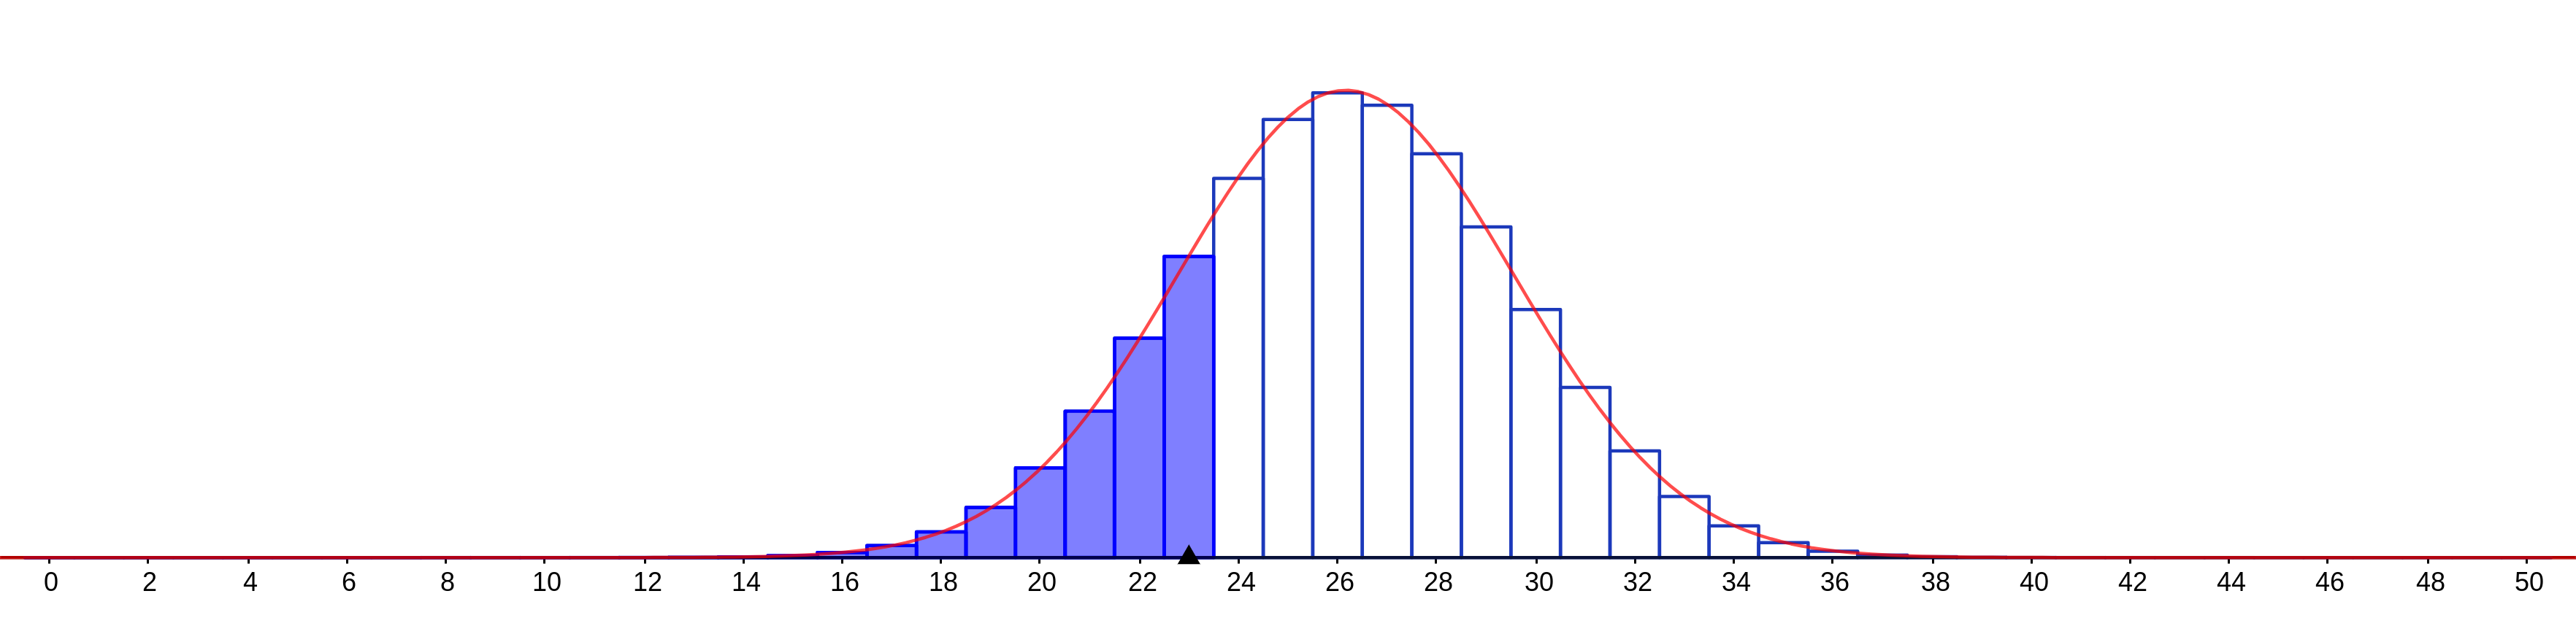
\includegraphics[width=0.5\linewidth]{pics/g13-1}
		\centering
	\end{figure}\noindent
	y una $P(X\geq 30) = 0.1621$  con el gráfico:
	\begin{figure}[H]
		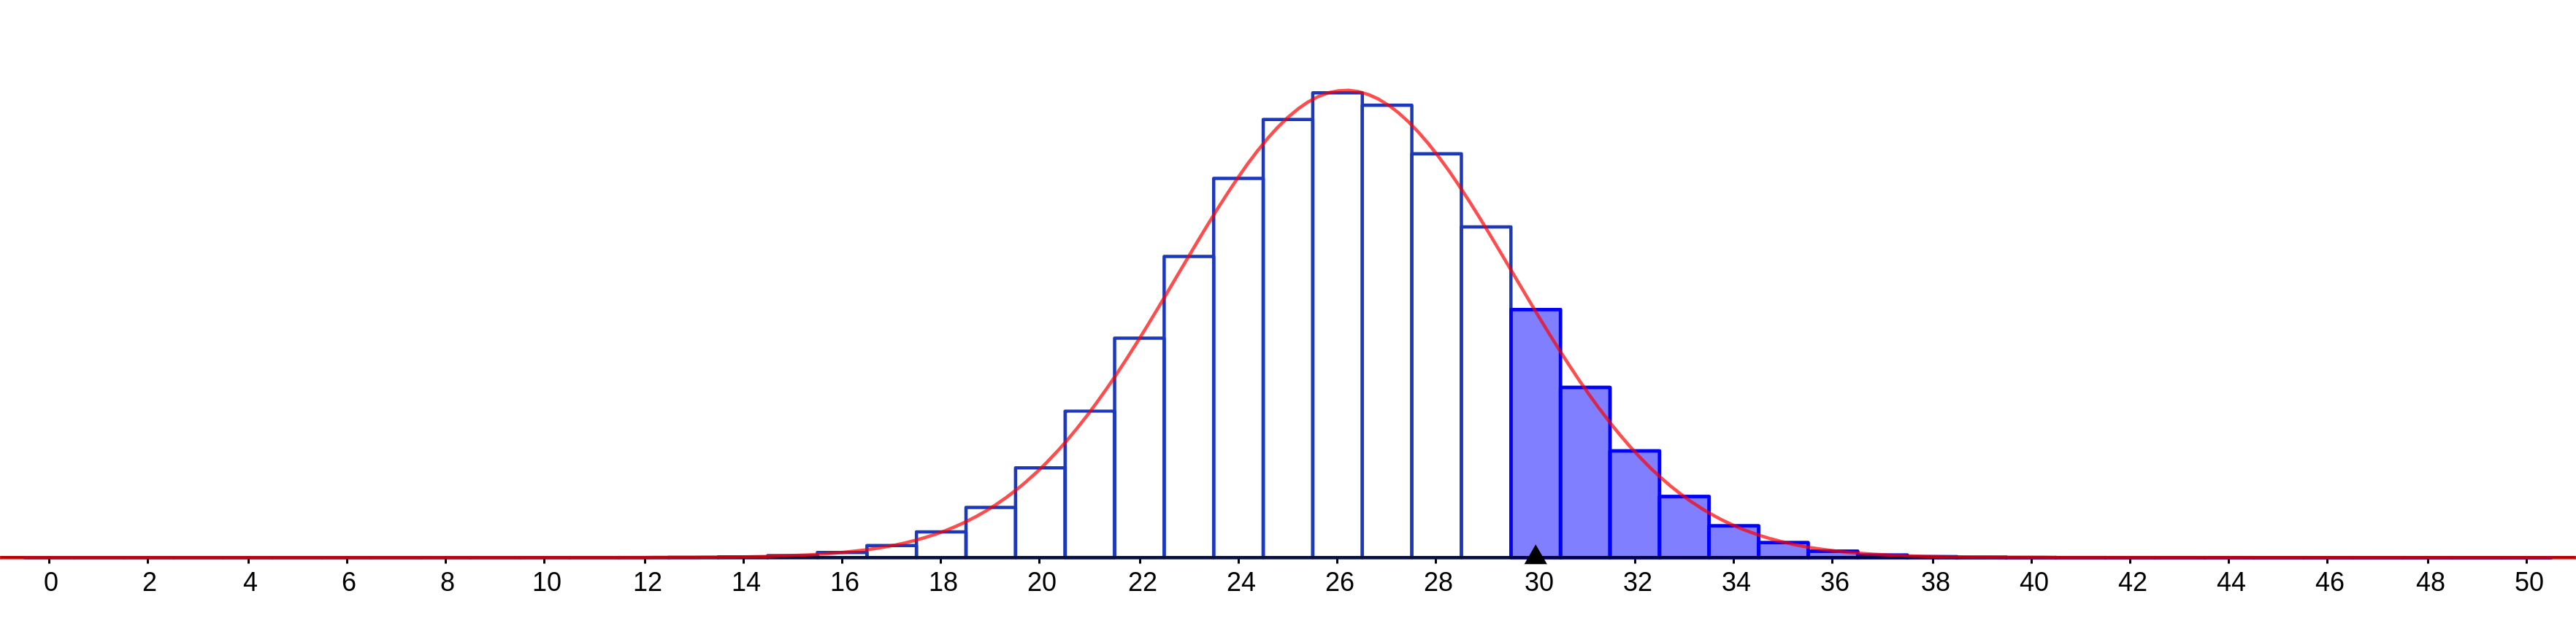
\includegraphics[width=0.5\linewidth]{pics/g13-2}
		\centering
	\end{figure}\noindent
	Por otro lado, en \texttt{R}, $P(X\leq 23)$ es:
	\begin{lstlisting}[language=R]
> phyper(23, 314, 600-314, 50, lower.tail = TRUE)
[1] 0.2150751
	\end{lstlisting}
	y la $P(X\geq 30)$ es:
	\begin{lstlisting}[language=R]
> phyper(29, 314, 600-314, 50, lower.tail = FALSE)
[1] 0.1621491
	\end{lstlisting}
\end{sol}
\end{document}